%% A chapter for my PhD dissertation
%% First author: Theodore Pak
%%
%% Must be included from main.tex.

\chapter{Mass cytometry and transcriptomics of the innate immune response to chikungunya infection reveals a central role for monocytes}
\label{chap:chik}

\hyphenation{Me-ta-Hy-brid-Lou-vain Wi-ki-Path-ways Wil-cox-on strong-ly che-mo-kines}
\newcommand{\subcommunity}{sub-\allowbreak com\-mu\-ni\-ty}
\newcommand{\subcommunities}{sub-\allowbreak com\-mu\-ni\-ties}
\newcommand{\Subcommunities}{Sub-\allowbreak com\-mu\-ni\-ties}
\newcommand{\pertranscript}{per-\allowbreak trans\-cript}

\sidequote{\smallcaps{Agent Smith}, \emph{The Matrix}}{
  I'd like to share a revelation that I've had during my time here. It came to me when I tried to classify your species and I realized that you're not actually mammals. Every mammal on this planet instinctively develops a natural equilibrium with the surrounding environment but you humans do not. You move to an area and you multiply and multiply until every natural resource is consumed and the only way you can survive is to spread to another area. There is another organism on this planet that follows the same pattern. Do you know what it is? A virus. Human beings are a disease, a cancer of this planet. You're a plague and we are the cure.
}

\sidequote{\smallcaps{Jonas Salk}}{
  I pictured myself as a virus, or a cancer cell, and tried to sense what it would be like.
}

\begin{quote}
\emph{Chikungunya virus (CHIKV) is a globally epidemic mosquito-borne alphavirus causing acute and chronic arthritic disease. Our study used a systems immunology approach by incorporating whole blood RNA-seq, 35-plex mass cytometry of PBMCs, and serum cytokine measurements of acute and convalescent phase samples from 42 natural pediatric infections in Nicaragua. Semi-supervised classification and clustering of single-cell events into 57 \subcommunities{} of canonical leukocyte phenotypes revealed a monocyte-driven response to acute infection, with greatest expansions of “intermediate” CD14\sups{++}\allowbreak CD16\sups{+} monocytes and an activated subpopulation of CD14\sups{+} monocytes. Increases in acute phase CHIKV surface protein expression were highest for monocytes and dendritic cells, although surprisingly, B cell subpopulations also displayed significant increases. Serum cytokine measurements confirmed significant acute phase upregulation of monocyte chemoattractants. Transcriptomic signatures were revealed not only for infection phase, but also for convalescent phase immunogenicity, acute phase viremic load, and symptom severity. Finally, we present a multiscale network that summarizes all observed modulations across cellular and gene expression levels and their interactions with clinical outcomes, providing a uniquely global view of the biomolecular landscape of CHIK pathophysiology.}
\end{quote}

\newthought{Chikungunya} (CHIKV) is a re-emerging mosquito-borne alphavirus that causes endemic and explosively epidemic infections throughout tropical regions of the world.\autocite{Weaver2015} Transmittable by \emph{Aedes egypti} and \emph{Aedes albopictus}, the same vectors as Dengue virus (DENV), phylogenies of CHIKV have indicated that urban endemic strains originated from several transmission events out of enzootic, sylvatic cycles between non-human primates and arboreal mosquitos in eastern Africa.\autocite{Volk2010} In 2004, the largest outbreak ever recorded spread rapidly from Africa through the Indian Ocean and Asia to Papua New Guinea and islands in the Pacific; subsequently, the first autochthonus transmissions in the Americas and the US were reported in 2013.\autocite{Nasci2014} Millions of cases have now been reported in at least forty countries.\autocite{Suhrbier2012}

Unlike other arboviral diseases like DENV, the majority of CHIKV infections produce symptomatic illness, with typical manifestations consisting of fever, a diffuse body rash, and joint pain and inflammation.\autocite{Couderc2015,Weaver2015} Notably, debilitating joint-related symptoms can persist for years mimicking rheumatoid arthritis in up to 50\% of afflicted populations—the namesake characteristic of the disease, as “chikungunya” is a Swahili/Makonde word describing a bent posture.\autocite{Miner2015,Weaver2015} Rarely, complications can occur, including encephalopathy and encephalitis, fulminant hepatitis, and myocarditis.\autocite{Rolph2015} Mortality occurs in approximately 0.1\% of cases.\autocite{Rolph2015} Besides anti-inflammatories for symptomatic relief, there are no specific treatments available for CHIKV.\autocite{Suhrbier2012,Weaver2015} Several vaccine candidates have reached preclinical or phase I trials,\autocite{Plante2015,Weger-Lucarelli2014} but major commercial investment will be required to complete their development, and finding clinical sites to demonstrate efficacy will be complex because of the unpredictable incidence and spread of the virus.\autocite{Weaver2015} Until a vaccine or antiviral agent is available, prevention efforts will remain focused on mosquito control.\autocite{Weaver2015}  

Because of CHIKV’s recent re-emergence in the Western hemisphere, there are profound gaps in the understanding of CHIKV pathogenesis, including uncertainty over the roles of viral proteins and the myriad genetic and signaling factors involved in a successful or unsuccessful immune response,\sidecite[-1cm]{Assuncao-Miranda2013,Sourisseau2007,Weaver2015} particularly in pediatric cases.\autocite{Teng2015} CHIKV can infect many cell types, including skin fibroblasts, endothelial cells, primary epithelia, and human muscle satellite cells.\autocite{Couderc2015,Lum2015} Reports of tropism in subsets of peripheral blood monocytes (PBMCs) vary, with CHIKV antigens detected in monocytes during acute infection,\autocite{Her2010} although primary monocytes and macrophages only appear to be infectable at low efficiency in vitro.\autocite{Sourisseau2007,Teng2012a} Thus far, primary B and T cells have not been successfully infected in vitro.\autocite{Her2010,Sourisseau2007,Teng2012a} Monocytes and macrophages are thought to have a substantial role in the acute inflammatory response to CHIKV, as primate models show consistent recruitment of these cell types and natural killer (NK) cells into infected tissues,\autocite{Labadie2010} and mouse models treated with bindarit (an inhibitor of monocyte chemoattractant CCL2) showed reduced monocyte recruitment, joint swelling, and bone loss following infection.\autocite{Chen2015,Rulli2011} The role of monocytes appears to be protective as well as inflammatory. For example, mice deficient for CCR2 (the receptor for CCL2) show prolongation of arthritic disease corresponding with replacement of the monocyte/macrophage infiltrate in infected joints by neutrophils and eosinophils.\autocite{Poo2014} In humans, however, details of the relationship between monocyte subpopulations, acute phase pathogenesis, and chronic symptomatology remain poorly understood.\autocite{Burt2017,Weaver2015}

The innate immune response, particularly via type I interferon (IFN) signaling, is important for control of CHIKV replication during the acute phase of infection.\autocite{Burt2017,Schilte2010} CHIKV infection acutely induces high levels of IFNα release in both humans and model organisms.\autocite{Labadie2010,Teng2015} In mouse models, type I IFNs control CHIKV replication by directly acting on nonhematopoietic cells, likely via activation of host sensors for viral RNA, such as RIG-I and MDA5.\autocite{Schilte2010} Additionally, either IRF-3 or IRF-7 signaling appears to be independently sufficient for preventing lethality of CHIKV infection in adult mice.\autocite{Schilte2012} In primary cell culture and mice, interferon stimulated genes such as the OAS family and RSAD2 (Viperin) appear to exert antiviral roles against CHIKV, although the details of these signal transduction pathways and their relative importance are unresolved.\autocite{Burt2017}

\newthought{Historically, the immune system} has been described by evaluating individual components in isolation. This approach is often biased toward better-recognized phenotypes and pathways and is likely to miss globally significant patterns of interconnectivity, particularly across the multiple conjoint scales of the immune system, e.g., transcriptional modulation within cells, resultant expansion and contraction of certain cell populations, and crosstalk between those immune cells and disparate tissues.\autocite{Kidd2014} Genome-wide expression profiling using microarrays or RNA-seq and mass cytometry using Cytometry by Time-of-Flight (CyTOF) offer the capability to perform unbiased, systematic exploration of hundreds of thousands of changes transpiring within a particular perturbation of the immune system. Weighted coexpression and probabilistic causal network models can then synthesize data from “omic” assays into a map of quantitative relationships between all regulatory elements of a particular immune response, which is one of the goals of systems immunology.\sidecite[-2cm]{Arazi2013,Germain2011} Although biomolecular network models have demonstrated utility in finding causal gene modules and novel mechanisms for complex, inheritable human diseases,\sidecite[-1cm]{Chen2008,Emilsson2008,Huan2015,Zhang2013} because of the difficulty in acquiring data at the scale necessary for fitting these models, they remain relatively new in the field of infectious diseases. Even still, network models have already helped map detailed regulatory circuits in hematopoiesis, transcriptional regulation of hundreds of leukocyte populations in mice, and viral sensing mechanisms in dendritic cells via Toll-like receptors (TLRs).\autocite{Kidd2014}

Previous observational studies of the immune response to CHIKV in natural human infections typically concentrated on protein or gene expression levels of a small number of cytokines and inflammatory mediators,\autocite{Chaaitanya2011,Chow2011,Kelvin2011,Ng2009,Teng2015} often producing conflicting results.\autocite{Burt2017} Among studies that used cytometry, one group employed CyTOF to profile ten CHIKV patients, but their analysis focused almost entirely on T cells.\autocite{Miner2015} Our study, by contrast, employs a systems immunology approach, integrating three high-throughput techniques to comprehensively profile the acute and convalescent phases of 42 pediatric cases of natural CHIKV infection in Managua, Nicaragua. To our knowledge, we provide here the first published RNA-seq study of CHIKV infection in humans, the first report of CHIKV-induced modulations for nearly all peripheral blood mononuclear cell (PBMC) subpopulations in humans, and the only study that applies multiple molecular profiling techniques to pediatric cases of CHIKV. We used whole blood samples from patients visiting an acute care facility that were lab-confirmed as cases of CHIKV viremia, comparing each patient’s acute phase sample (1-2 days post symptom onset [p.s.o.]) against paired samples taken two weeks later, after resolution of symptoms and viremia. We analyzed these samples using CyTOF, RNA-seq, and multiplex ELISA (Luminex), employing a systematic, hypothesis-free approach for finding globally significant changes in cell subpopulation frequencies, gene expression, and serum cytokine concentrations during acute CHIKV infection. We then searched for interactions within all of these data and with measurements of clinical outcomes such as the viral titer during the acute phase, the severity of symptoms at presentation, and the convalescent phase CHIKV immunoglobulin G (IgG) titer. Finally, to synthesize these interactions across the three examined scales, we present a multiscale network model that summarizes all correlations between gene modules, cell subpopulations, and clinical variables in this study.

\begin{table}[tbp]
  \centering
\small
\begin{tabular}{l l}
  \toprule
  Phenotype/covariate &
  Participants (\emph{N}=42)\\
  \midrule
  Gender
  \\
  \-\tabindent Female, no. (\%) &
  11 (26)
  \\
  \-\tabindent Male, no. (\%) &
  31 (74)
  \\
  Age
  \\
  \-\tabindent Years, mean ± SD &
  9.22 ± 4.5
  \\
  \-\tabindent 1-4 years old (\%) &
  9 (21)
  \\
  \-\tabindent 5-8 years old (\%) &
  9 (21)
  \\
  \-\tabindent 9-14 years old (\%) &
  23 (57)
  \\
  Signs or symptoms at enrollment &
  \\
  \-\tabindent Days post symptom onset, mean ± SD &
  1.41 ± 0.5
  \\
  \-\tabindent Fever, mean temperature ± SD, °C &
  38.3 ± 0.8
  \\
  \-\tabindent Fever, mean duration ± SD, days &
  2.4 ± 0.6
  \\
  \-\tabindent Peak fever >38.5°C (\%) &
  16 (38)
  \\
  \-\tabindent Retroorbital pain (\%) &
  7 (16)
  \\
  \-\tabindent Osteomuscular pain (\%) &
  26 (62)
  \\
  \-\tabindent Rash (\%) &
  41 (98)
  \\
  \-\tabindent Arthralgia (\%) &
  36 (86)
  \\
  \-\tabindent Myalgia (\%) &
  20 (48)
  \\
  \-\tabindent Headache (\%) &
  9 (21)
  \\
  \-\tabindent Abdominal pain (\%) &
  13 (31)
  \\
  \-\tabindent Vomiting (\%) &
  4 (10)
  \\
  \-\tabindent Fluid accumulation (\%) &
  14 (33)
  \\
  \-\tabindent Hospitalized (\%) &
  36 (86)
  \\
  Laboratory values at enrollment &
  \\
  \-\tabindent Median platelet count, mm\sups{-3} (range) &
  199,000 (88,000–337,000)
  \\
  \-\tabindent Nadir platelet count <100,000 mm\sups{-3} (\%) &
  8 (19)
  \\
  \-\tabindent Median white cell count, mm\sups{-3} (range) &
  8,140 (3,030–16,120)
  \\
  \-\tabindent Median monocyte \% of WBCs (range) &
  8.9 (4.1–14.6)
  \\
  \-\tabindent Median lymphocyte \% of WBCs (range) &
  39.7 (10.4–66.4)
  \\
  Laboratory values at convalescent timepoint &
  \\
  \-\tabindent Days post symptom onset, mean ± SD &
  15.7 ± 0.6
  \\
  \-\tabindent Median CHIKV IgG Ab titer, dilutions (range) &
  1,458 (232–7,794)
  \\
  Severity categorization$^a$ &
  \\
  \-\tabindent Severe (\%) &
  21 (50)
  \\
  \-\tabindent Non-severe (\%) &
  21 (50)
  \\
  \bottomrule
\end{tabular}
  \caption[Clinical characteristics of study population]{\textbf{Clinical characteristics of study population.} Abbreviations: WBC, white blood cell; CHIKV, chikungunya virus; IgG, immunoglobulin G; Ab, antibody.
  \captionfootnotetext{a}{Cases were categorized as severe if the patient had either a peak fever of >38.5°C or a nadir platelet count of <100,000 mm\sups{-3}.}
}
  \label{tab:chik_pts}
\end{table}

\section{Results}

\subsection{Clinical characteristics of study participants}

Blood samples for this study were collected from the Nicaraguan National Pediatric Reference Hospital in Managua, Nicaragua during routine care. Patients were sampled and tested following presentation with symptoms and histories suggestive of DENV or CHIKV infection, and a diagnosis of CHIKV viremia was confirmed by either RT-PCR or viral isolation assay. A total of 42 pediatric cases of CHIKV viremia presenting between November 2014 and October 2015 were included, from which acute (1-2d p.s.o.) and convalescent (15-17d p.s.o.) samples were obtained, for a total of 84 samples.
De-identified clinical data were obtained for all samples and are summarized in Table \ref{tab:chik_pts}. 74\% of the patients were male, and over half were between 9-14 years of age. Rash was the most common presenting symptom (41/42, 98\%), followed by arthralgia (36/42, 86\%). Most of the patients were febrile (mean temperature, 38.3°C) and the average fever duration was 2.4 days. Of the cases studied, 36/42 (86\%) resulted in hospitalization. We adapted a previous rubric for classifying CHIKV cases as non-severe vs.\ severe.\autocite{Chow2011,Ng2009} In this study, a severe case is defined by a peak temperature >38.5°C or a nadir platelet count <100,000 mm\sups{-3}. By this criterion, half of the pediatric cases (21/42, 50\%) were considered severe.

\begin{figure}[htb]
  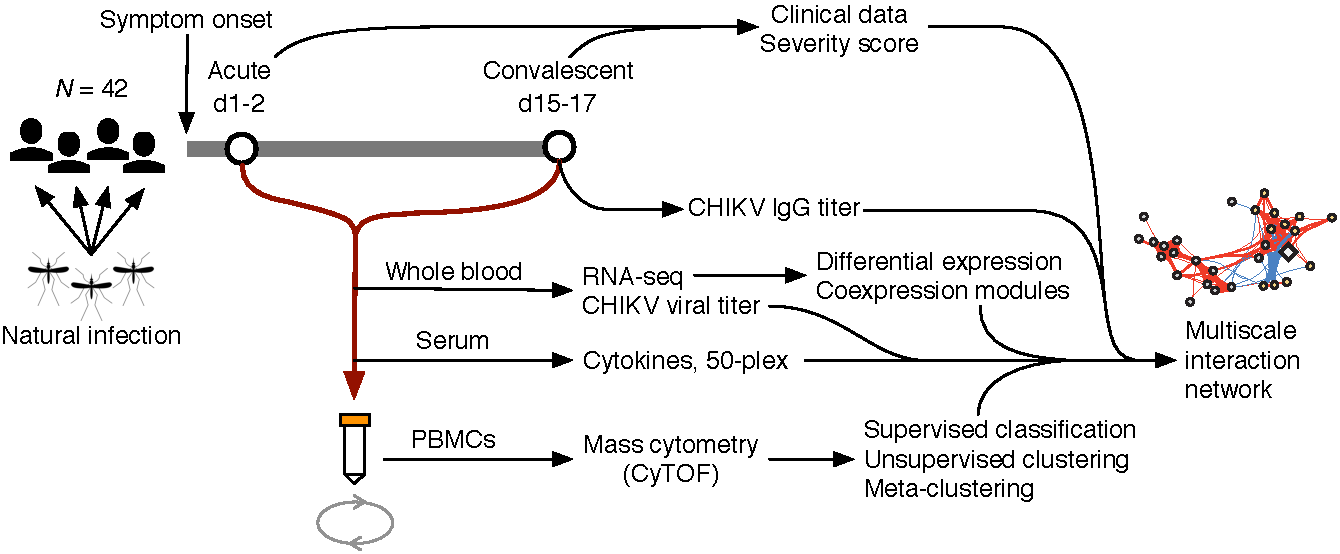
\includegraphics[width=\textwidth]{chap6/fig_1_study_design}
  \caption[Chikungunya immune profiling study design]{\textbf{Study design.} Blood samples were obtained from 42 pediatric cases of natural chikungunya (CHIKV) infections at an acute (d1-2) and a convalescent (d15-17) timepoint, relative to reported symptom onset. Samples were separated into whole blood, serum, and peripheral blood mononuclear cell (PBMC) aliquots for transcriptomic analysis, CHIKV viral titer assays, multiplex ELISA for cytokines, and mass cytometry (CyTOF), respectively. These data were combined with clinical data, including a severity score and a d15-17 CHIKV immunoglobulin G (IgG) titer, to create a multiscale network of interactions during the observed course of CHIKV infection.
  }
  \label{fig:chik_study_design}
\end{figure}

Sampling times closely adhered to the targeted acute (SD = 0.5d) and convalescent (SD = 0.6d) timepoints. Each blood sample was separated into aliquots of whole blood, serum, and PBMCs for transcriptomic analysis via RNA-seq, CHIKV viral titer assays, multiplex ELISA for cytokines, and mass cytometry as illustrated in Figure \ref{fig:chik_study_design}. These data were then analyzed for changes correlating with the acute and convalescent phases of infection, severe and non-severe cases, the 15d immunoglobulin G (IgG) titer, and the acute phase viral titer. The resulting signatures and clusters were combined into a multiscale interaction network capturing the global landscape of immune responses to CHIKV.

\subsection{Acute infection associates with CD14\sups{+}\allowbreak CD16\sups{+} monocyte expansion}

\begin{figure*}[htb]
  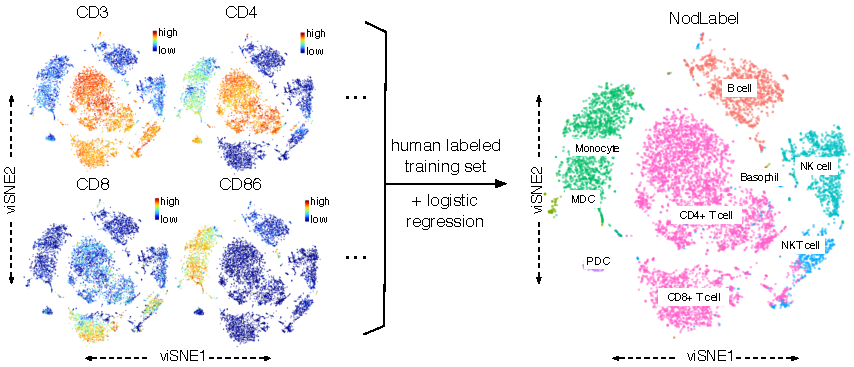
\includegraphics[width=\textwidth]{chap6/fig_2a_nodlabel_diag}
  \caption[Overview of the \texttt{NodLabel} procedure]{\textbf{Overview of the \texttt{NodLabel} procedure}, using a viSNE layout of CyTOF single-cell events. Left side, point color indicates channel values for four example channels. Right side, traditional hierarchical gating was used on a subset of samples to identify 9 major immune compartments, which was then used to train a logistic regression classifier (Nod) that applied labels for canonical leukocyte phenotypes to all samples (NodLabel).
  }
  \label{fig:nodlabel_diag}
\end{figure*}

CyTOF uses metal-labeled reagents and inductively coupled plasma mass spectrometry to overcome the limits of fluorescence spectral overlap in flow cytometry, allowing measurement of up to 50 analytes at single-cell resolution. We used CyTOF to quantify 35 immune cell surface markers (Appendix Table \ref{tab:chik_antibodies}) and the CHIKV surface protein in each of our samples. The high dimensionality of CyTOF data presents challenges for applying the traditional gating methods used in lower-dimensional flow cytometry. To address these challenges, we developed a sequential, semi-supervised approach to identify and classify immune cell populations in the CyTOF dataset. Manual gating and human-authored labels were first applied to a subset of the data to train a logistic regression classifier (called \texttt{NodLabel}) that was run on the remaining samples to broadly define 9 major immune subsets in each of the patient samples. Figure \ref{fig:nodlabel_diag} illustrates this process using a viSNE layout algorithm\autocite{Amir2013} for 2D visualizations of high-dimensional CyTOF data from a representative patient sample.

To define additional heterogeneity within each of these broad subsets, we next applied Louvain/Phenograph\autocite{Levine2015a} as an unsupervised clustering method to each \texttt{NodLabel}-identified subset in each patient sample.
\begin{figure*}[htb]
  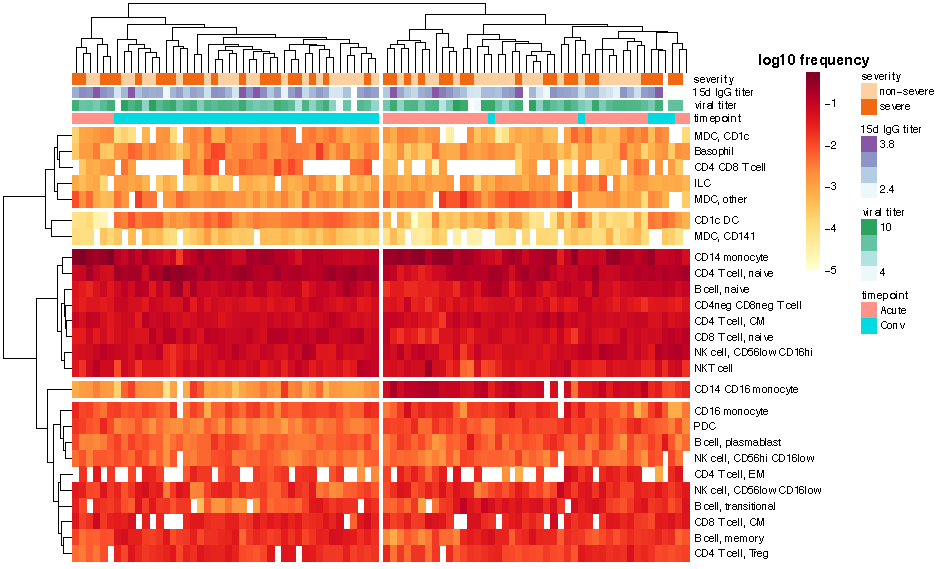
\includegraphics[width=\textwidth]{chap6/fig_2b_comm_heatmap}
  \caption[CyTOF signatures for acute CHIKV infection based on canonical immune cell phenotypes]{\textbf{CyTOF reveals signatures for acute CHIKV infection based on canonical immune cell phenotype clustering.} Heatmap of log\subs{10} scaled peripheral blood mononuclear cell (PBMC) community frequencies for all samples. Clinical variables are depicted for all samples across the top of the heatmap; 15d post symptom onset immunoglobulin G (IgG) titer and viral titer (which was measured during the acute phase) are both in units of log\subs{10} dilutions. Hierarchical clustering (using complete linkage) was applied to both samples (X axis) and communities (Y axis). Four major clusters of communities and two major clusters of samples (largely separating acute and convalescent samples) are highlighted. 
  }
  \label{fig:comm_heatmap}
\end{figure*}
While the combination of the \texttt{NodLabel} classifier and Phenograph (which we term \texttt{HybridLouvain}) is a powerful approach to define phenotypic heterogeneity in a sample, a limitation of the approach is that the identified \texttt{HybridLouvain} communities are only applicable to a single patient sample. To address this issue, we meta-clustered the individual communities across all patient samples, and meta-communities that were reproducibly identified across multiple patients were then manually annotated based on overall marker expression patterns. These annotations were then mapped back to each individual patient sample to provide consistent community definitions across all samples. Using this approach (which we term \texttt{MetaHybridLouvain}) we identified 26 communities of canonical leukocyte populations across all acute and convalescent phase samples (Figure \ref{fig:comm_heatmap}).
\begin{figure*}[htb]
  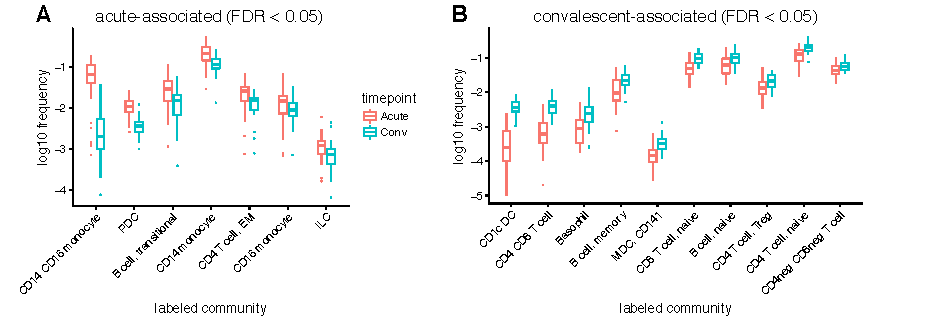
\includegraphics[width=\textwidth]{chap6/fig_2c_comm_diffs}
  \caption[PBMC communities with differing frequency across the CHIKV infection phases][-0.7cm]{\textbf{PBMC communities with differing frequency across the timepoints of CHIKV infection.} A, log\subs{10} frequencies for PBMC communities contrasted between acute and convalescent phase samples, filtered to communities where the acute phase frequency was higher at a significance threshold of FDR < 0.05 (Mann-Whitney \emph{U}). B, same as A but filtered to communities where the convalescent phase frequency was higher at a significance threshold of FDR < 0.05.
  }
  \label{fig:comm_diffs}
\end{figure*}
Hierarchical clustering by sample revealed two clusters that generally separated by timepoint, with no communities corresponding to any apparent contrasts in severity, 15d IgG titer, or acute phase viral titer (Figure \ref{fig:comm_heatmap}). Clustering by community frequency reveals a distinct contrast in CD14\sups{+}\allowbreak CD16\sups{+} monocyte frequencies between the acute and convalescent phases (vertical axis, Figure \ref{fig:comm_heatmap}). This is the most expanded population at the acute timepoint (Figure \ref{fig:comm_diffs}A), and the difference was highly significant (Bonferroni-corrected [BF] \emph{P} = 1.9e-09). Other populations also comparatively upregulated during the acute phase were plasmacytoid dendritic cells (PDCs) (BF \emph{P} = 4.7e-13) and CD14\sups{+} monocytes (BF \emph{P} = 0.0019), with four additional populations identified at a threshold false discovery rate (FDR) < 0.05 (Figure \ref{fig:comm_diffs}A). Ten populations were comparatively downregulated at the acute phase and thereby convalescent-associated at FDR < 0.05 (Figure \ref{fig:comm_diffs}B), with the strongest difference being observed in CD1c dendritic cells (DCs) (BF \emph{P} = 3.9e-19).

\subsection{Monocytes, dendritic cells, and B cells express CHIKV surface protein during acute infection}

\begin{marginfigure}[-2cm]
  \centering
  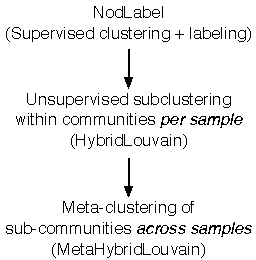
\includegraphics[width=0.7\textwidth]{chap6/fig_3a_mhl_diag}
  \vspace{1em}
  \caption[Overview of the \texttt{MetaHybridLouvain} procedure]{Overview of the \texttt{MetaHybridLouvain} procedure.}
  \label{fig:mhl_diag}
\end{marginfigure}

Classifying CyTOF events into only the canonical leukocyte populations ignores much of the richness of these data, which can reveal previously unrecognized diversity and heterogeneity within each of these populations. The advantage of our \texttt{MetaHybridLouvain} approach (Figure \ref{fig:mhl_diag}) is that it allows for unbiased identification of phenotypically heterogenous \subcommunities{} within each of the canonical immune subsets,\footnote[][-1.5cm]{As opposed to strict classification methods, e.g. \textcite{Lee2017}, which require pre-defining all desired cell types. A complete comparison of CyTOF classification and clustering methods is beyond this chapter's scope, but \textcite{Aghaeepour2013} provides an introduction, and \textcite{Samusik2016} is a comparable clustering method that also emphasizes novel subpopulation discovery.} e.g., a \subcommunity{} of CD14\sups{+} monocytes as defined by a specific, reproducible marker expression pattern across multiple samples. This allowed for the identification of up to nine \subcommunities{} within certain defined canonical immune populations (Figure \ref{fig:mhl_visne}, \ref{fig:mhl_subcomms}), producing a total of 57 \subcommunities{}. More detailed results of \texttt{Me\-ta\-Hy\-brid\-Lou\-vain} for the representative sample used in Figure \ref{fig:nodlabel_diag} and \ref{fig:mhl_visne} are depicted in Appendix Figures \ref{fig:mhl_example}-\ref{fig:mhl_example_cont}.

\begin{figure}[htb]
  \centering
  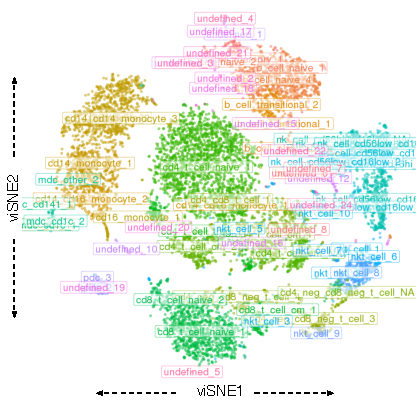
\includegraphics[width=0.8\textwidth]{chap6/fig_3b_mhl_visne}
  \caption[viSNE layout of \texttt{MetaHybridLouvain} \subcommunities{}]{viSNE layout of CyTOF single-cell events from the same representative sample as Figure \ref{fig:nodlabel_diag}, now with labels for peripheral blood mononuclear cell (PBMC) \subcommunities{} detected by \texttt{MetaHybridLouvain} drawn at the centroid of each \subcommunity{}.
  }
  \label{fig:mhl_visne}
\end{figure}
\begin{marginfigure}
  \centering
  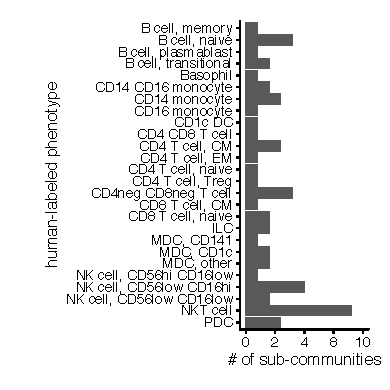
\includegraphics[width=\textwidth]{chap6/fig_3c_mhl_subcomms}
  \caption[Number of \subcommunities{} detected by \texttt{MetaHybridLouvain} per canonical phenotype]{Number of \subcommunities{} detected by \texttt{MetaHybridLouvain} for each of the canonical leukocyte phenotypes.}
  \label{fig:mhl_subcomms}
\end{marginfigure}

Having dissected the cellular heterogeneity of the samples at high resolution, we went on to identify leukocyte populations that have comparatively high levels of CHIKV surface protein during the acute phase of infection. Qualitatively, in the representative patient sample, CHIKV surface protein was expressed by distinct populations of leukocytes in the viSNE layout (Figure \ref{fig:chikv_visne})—in particular monocytes, dendritic cells, and B cells (compare with Figures \ref{fig:nodlabel_diag} and \ref{fig:mhl_visne}). Quantitatively, across all samples, monocytes and dendritic cells displayed the strongest contrasts in mean CHIKV channel values per sample between acute and convalescent timepoints (Figure \ref{fig:chikv_diffs}).
\begin{figure}[htb]
  \centering
  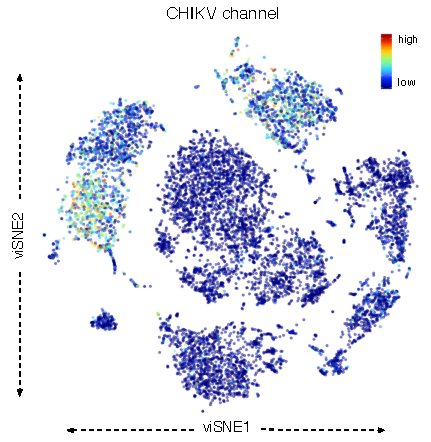
\includegraphics[width=0.8\textwidth]{chap6/fig_3d_chikv_visne}
  \caption[viSNE layout of CHIKV surface protein expression levels]{viSNE layout of CyTOF single-cell events from the same representative sample as Figure \ref{fig:nodlabel_diag} and \ref{fig:mhl_visne}, now with points colored according to the CHIKV channel. By qualitative comparison with Figure \ref{fig:nodlabel_diag} (reproduced below), monocytes, myeloid dendritic cells (MDCs), and B cells have the highest CHIKV surface protein expression. 
  }
  \label{fig:chikv_visne}
\end{figure}
CHIKV-positive cell populations largely fell along canonical leukocyte phenotype boundaries, with all three \subcommunities{} of CD14\sups{+} monocytes (BF \emph{P} = 2.5e-26, 2.7e-24, 8.1e-16), both \subcommunities{} of CD1c MDCs (BF \emph{P} = 4.2e-15 and 4.3e-08), all CD1c DCs (BF \emph{P} = 4.3e-16), and both \subcommunities{} of CD14\sups{+}\allowbreak CD16\sups{+} monocytes (BF \emph{P} = 2.5e-09 and 2.3e-06) identified as significantly more CHIKV-positive during the acute phase. Interestingly, although the differences were less pronounced, three \subcommunities{} of B cells were also observed to express significantly higher CHIKV surface protein during acute infection: the only community of memory B cells (BF \emph{P} = 3.2e-09) and two of the four \subcommunities{} of naïve B cells (BF \emph{P} = 9.7e-06 and 0.00022). Although CHIKV surface protein expression only correlates with (and does not establish) tropism of the virus, our data suggest that among PBMCs, CHIKV preferentially infects monocytes and dendritic cells, while displaying lower but substantial affinity for B cells.

\begin{marginfigure}[-16cm]
  \centering
  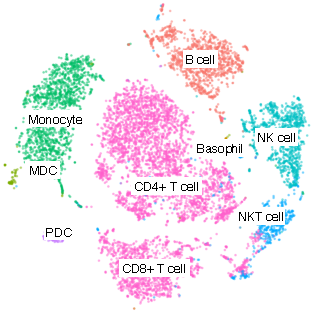
\includegraphics[width=\textwidth]{chap6/fig_2a-repeat_nodlabel_just_visne}
\end{marginfigure}

\begin{marginfigure}[-5cm]
  \centering
  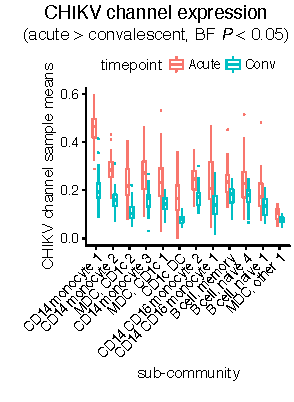
\includegraphics[width=\textwidth]{chap6/fig_3e_chikv_diffs}
  \caption[Number of \subcommunities{} detected by \texttt{MetaHybridLouvain} per canonical phenotype]{Differences in CHIKV surface protein expression between acute phase and convalescent phase samples per \texttt{MetaHybridLouvain} \subcommunity. \Subcommunities{} are ordered by largest to smallest difference and filtered to \subcommunities{} where the median of the channel means per sample was higher in the acute phase samples at a significance threshold of Bonferroni \emph{P} < 0.05. \Subcommunities{} are named by their parent canonical community name plus an arbitrary number, up to the counts given in Figure \ref{fig:mhl_subcomms}.}
  \label{fig:chikv_diffs}
\end{marginfigure}

\subsection{CD14\sups{+} and CD14\sups{+}\allowbreak CD16\sups{+} monocyte \subcommunities{} exhibit contrasting behaviors during acute infection}

\begin{figure*}[p]
  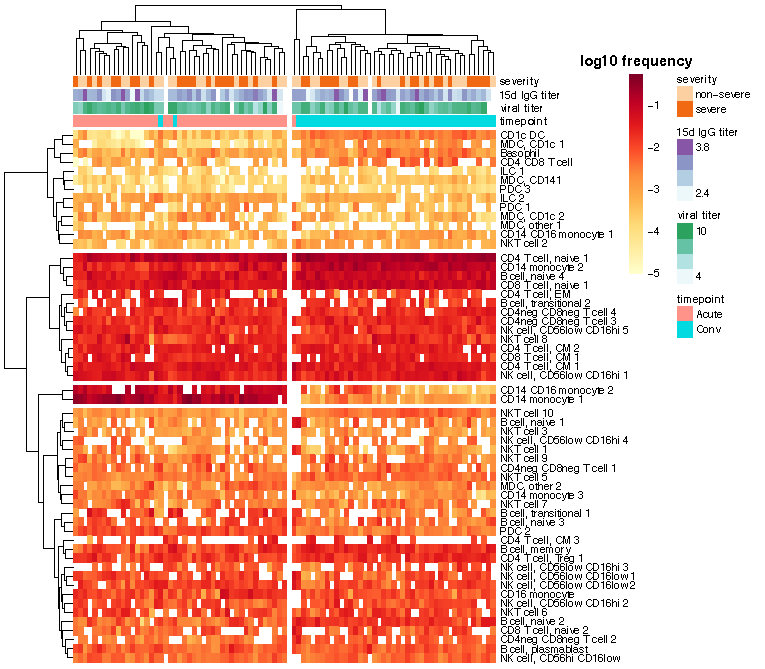
\includegraphics[width=\textwidth]{chap6/fig_3f_mhl_subcomm_heatmap}
  \fullwidthlabelcaption{fig:subcomm_heatmap}{Specific monocyte \subcommunities{} undergo expansion during acute CHIKV infection}{
  \textbf{Specific monocyte \subcommunities{} undergo expansion during acute CHIKV infection.} Heatmap of log\subs{10} scaled PBMC \subcommunity{} frequencies for all samples. Clinical variables are depicted for all samples across the top of the heatmap; 15d post symptom onset immunoglobulin G (IgG) titer and viral titer (which was measured during the acute phase) are both in units of log\subs{10} dilutions. Hierarchical clustering (using complete linkage) was applied to both samples (X axis) and \subcommunities{} (Y axis). Four major clusters of \subcommunities{} and two major clusters of samples (largely separating acute and convalescent samples) are highlighted. 
  }
\end{figure*}

Although CD14\sups{+}\allowbreak CD16\sups{+} monocytes expand during the acute phase of infection, community subclustering provides more detail on particular \subcommunities{} that associate with the acute phase. Hierarchical clustering of samples by \subcommunity{} frequencies separates the samples by timepoint more effectively than canonical population frequencies alone (Figure \ref{fig:subcomm_heatmap}, compare with Figure \ref{fig:comm_heatmap}), with only 3/88 (3\%) of samples misclassified between the two major clusters. Again, however, there was no apparent clustering of samples that corresponded to contrasts in clinical severity, 15d IgG titer, or acute phase viral titer. Stratifying by the acute and the convalescent phases, there were no significant differences
\begin{figure}[tb]
  \centering
  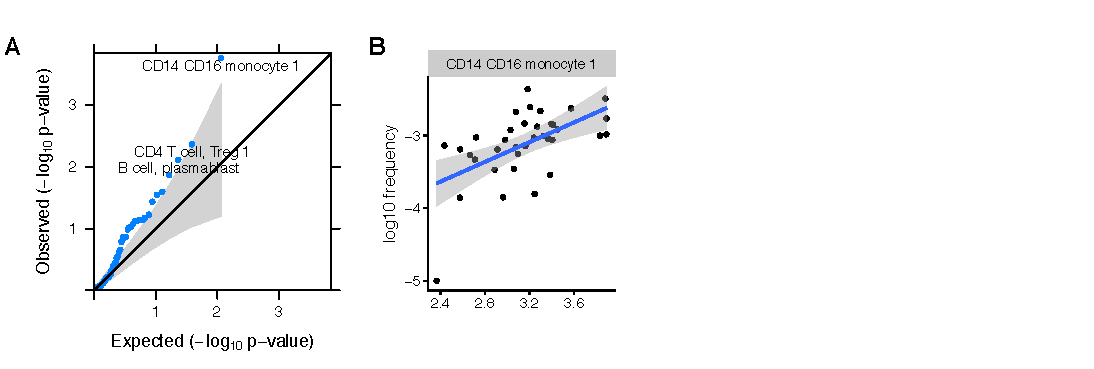
\includegraphics[width=0.88\textwidth]{chap6/fig_S2_corr_IgG_cd14cd16_mono_1}
  \caption[Correlations between acute phase cell \subcommunity{} frequencies and 15d CHIKV IgG titer]{
  \textbf{Correlations between acute phase cell \subcommunity{} frequencies and log\subs{10} CHIKV IgG titer at 15d post-symptom onset.} A, Q-Q plot of the distribution of observed –log\subs{10} \emph{P} values against the distribution of –log\subs{10} \emph{P} values expected under the null hypothesis (that Spearman’s $\rho = 0$ for all \subcommunities). Gray shaded band indicates the 95\% confidence interval for the expected \emph{P} value distribution under the null hypothesis. B, Scatterplots of log\subs{10} cell \subcommunity{} frequencies against log\subs{10} IgG CHIKV titer at the 15d timepoint for the CD14\sups{+}CD16\sups{+} monocyte 1 correlation, which is the only correlation significant after multiple hypothesis correction (BF \emph{P} = 0.0097, Spearman’s $\rho$ = 0.60).
  }
  \label{fig:corr_cytof_igg}
\end{figure}
in any \subcommunity{} frequencies between severe and non-severe cases at FDR < 0.1. Within either timepoint, there were also no significant correlations between \subcommunity{} frequencies and log-transformed acute phase viral titers at FDR < 0.1. There was, however, a single significant correlation between CD14\sups{+}\allowbreak CD16\sups{+} monocyte \subcommunity{} 1 at the acute phase and the 15d (convalescent) IgG titer
\begin{figure*}[htb]
  \centering
  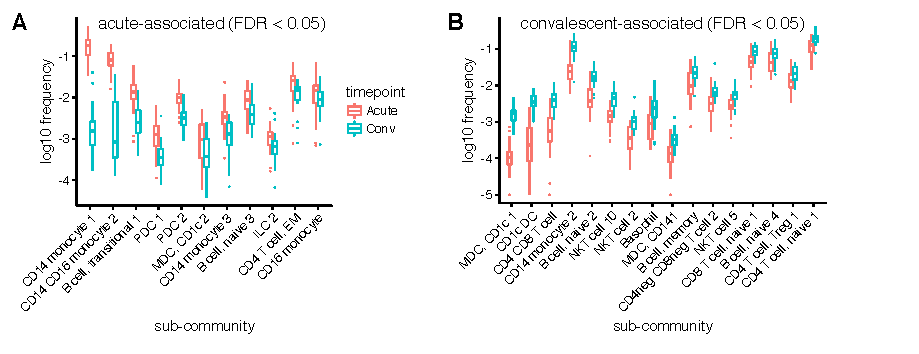
\includegraphics[width=0.95\textwidth]{chap6/fig_3g_subcomm_diffs}
  \caption[PBMC \subcommunities{} with differing frequency across the CHIKV infection phases]{
  \textbf{PBMC \subcommunities{} with differing frequency across the timepoints of CHIKV infection.} A, log\subs{10} frequencies for PBMC \subcommunities{} contrasted between acute and convalescent phase samples, filtered to \subcommunities{} where the acute phase frequency was higher at a significance threshold of FDR < 0.05 (Mann-Whitney \emph{U}). B, same as A but filtered to \subcommunities{} where the convalescent phase frequency was higher at a significance threshold of FDR < 0.05.
  }
  \label{fig:subcomm_diffs}
\end{figure*}
(BF \emph{P} = 0.0097, Spearman’s $\rho$ = 0.60; see Figure \ref{fig:corr_cytof_igg}), with no significant correlations among convalescent \subcommunity{} frequencies at FDR < 0.1.

Among \subcommunities{} significantly expanded during the acute phase, two particular expansions separated from the others by an order of magnitude (Figure \ref{fig:subcomm_diffs}A), specifically \subcommunity{} 1 of CD14\sups{+} monocytes (BF \emph{P} = 7.7e-21) and \subcommunity{} 2 of CD14\sups{+}\allowbreak CD16\sups{+} monocytes (BF \emph{P} = 2.8e-15).
\begin{figure*}[htb]
  \centering
  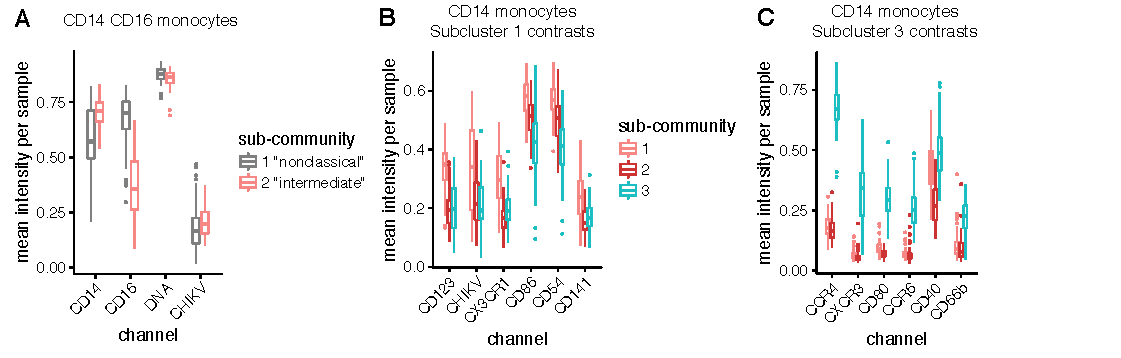
\includegraphics[width=0.95\textwidth]{chap6/fig_4_monocyte_subpops}
  \caption[Marker expression differences between sub-communities of CD14\sups{+}\allowbreak CD16\sups{+} monocytes and CD14\sups{+} monocytes]{
  \textbf{Marker expression differences between sub-communities of CD14\sups{+}\allowbreak CD16\sups{+} monocytes and CD14\sups{+} monocytes}, depicted as boxplots of the mean expression levels for all samples. A, relative expression of CD14\sups{+} and CD16\sups{+} in CD14\sups{+}CD16\sups{+} sub-communities indicates that sub-community 1 is a CD14\sups{+}CD16\sups{++} (aka “non-classical”) phenotype, while sub-community 2 is a CD14\sups{++}CD16\sups{+} (aka “intermediate”) phenotype. Differences shown here are significant at FDR < 0.05; for a view of all differences significant at this threshold, see Appendix Figure \ref{fig:cd14cd16_channel_diffs}. B, relative expression of six markers that most differentiate (by the difference in medians) sub-community 1 of CD14\sups{+} monocytes from the other sub-communities. C, relative expression of six markers that most differentiate (by the difference in medians) sub-community 3 of CD14\sups{+} monocytes from the other sub-communities. Note: Channels shown in B and C are a subset of the differences that are significant at FDR < 0.05; for a view of all differences significant at FDR < 0.05 see Appendix Figure \ref{fig:cd14_channel_diffs}.
  }
  \label{fig:subcomm_marker_diffs}
\end{figure*}
When examining the other two \subcommunities{} of CD14\sups{+} monocytes, one is also expanded during the acute phase but to a lesser extent (\subcommunity{} 3, BF \emph{P} = 5.6e-06) while the other instead is expanded during the convalescent phase (\subcommunity{} 2, BF \emph{P} = 1.6e-10). At FDR < 0.1, \subcommunity{} 1 of CD14\sups{+}\allowbreak CD16\sups{+} monocytes, which is the only other \subcommunity{} of CD14\sups{+}\allowbreak CD16\sups{+} monocytes, is not significantly different across timepoints. Other \subcommunities{} associating with the convalescent phase at FDR < 0.05 include MDCs, CD1c DCs, B cells, T cells, and basophils (Figure \ref{fig:subcomm_diffs}B).

Since different \subcommunities{} of CD14\sups{+}\allowbreak CD16\sups{+} and CD14\sups{+} monocytes displayed distinctive responses to acute CHIKV infection, we looked for marker differences that could better define these \subcommunities{}. Examination of the two CD14\sups{+}\allowbreak CD16\sups{+} monocyte \subcommunities{} (Figure \ref{fig:subcomm_marker_diffs}A) revealed that among all significant marker differences, \subcommunity{} 1 had higher CD16 expression (BF \emph{P} = 5.7e-19) and \subcommunity{} 2 had higher CD14 expression (BF \emph{P} = 6.4e-05). This corresponded to \subcommunities{} commonly called “nonclassical” CD14\sups{+}\allowbreak CD16\sups{++} and “intermediate” CD14\sups{++}\allowbreak CD16\sups{+} monocytes,\autocite{Wong2011,Ziegler-Heitbrock2010} implying that in our study, “intermediate” monocytes were substantially expanded during acute CHIK infection while “nonclassical” monocytes were unchanged. Significant contrasts in the expression of many other surface markers at FDR < 0.05 (Appendix Figure \ref{fig:cd14cd16_channel_diffs}) and the consistent identification of these patterns across the majority of samples (Appendix Figures \ref{fig:cd14cd16_subcomm_1_heatmap}-\ref{fig:cd14cd16_subcomm_2_heatmap}) confirmed the distinction between these \subcommunities{}.

Among the three \subcommunities{} of CD14\sups{+} monocytes, we discovered two that were associated with acute infection, including one with a previously unreported phenotype. \subcommunity{} 1 (the \subcommunity{} most strongly associated with acute infection and also expressing the highest levels of CHIKV surface protein) was characterized by having relatively higher levels of CD123, CX3CR1, CD86 and CD54 expression (Fig \ref{fig:subcomm_marker_diffs}B), generally consistent with a more activated phenotype relative to \subcommunity{} 2, which was more prevalent during convalescence. Monocyte \subcommunity{} 3 was also expanded during acute infection, though at a much lower frequency than monocyte \subcommunity{} 1, and displayed similar levels of CD40, consistent with an activated phenotype. Interestingly, however, this subset also exhibited comparatively high expression of markers that are not classically associated with monocytes, particularly the chemokine receptor CCR4, as well as CXCR3 and CCR6 (Figure \ref{fig:subcomm_marker_diffs}C). We further confirmed that this \subcommunity{} did not express canonical markers associated with other major cell types, such as T cells or B cells, to verify that it did not represent an artifact of cell-cell doublets. Again, significant contrasts in the expression of many surface markers at FDR < 0.05 (Kruskal-Wallis test, Appendix Figure \ref{fig:cd14_channel_diffs}), and a consistent pattern for the phenotype identified across the majority of samples (Appendix Figures \ref{fig:cd14_subcomm_1_heatmap}-\ref{fig:cd14_subcomm_3_heatmap}) confirmed the distinction between these \subcommunities{}. Given the strongly contrasting associations of these \subcommunities{} with the phase of infection, these data suggest that unappreciated heterogenity within CD14\sups{+} monocyte phenotypes may enable different roles for \subcommunities{} of these monocytes during CHIKV infection.  

\subsection{Monocyte-associated cytokine concentrations increase during acute infection}

\begin{figure*}[htb]
  \centering
  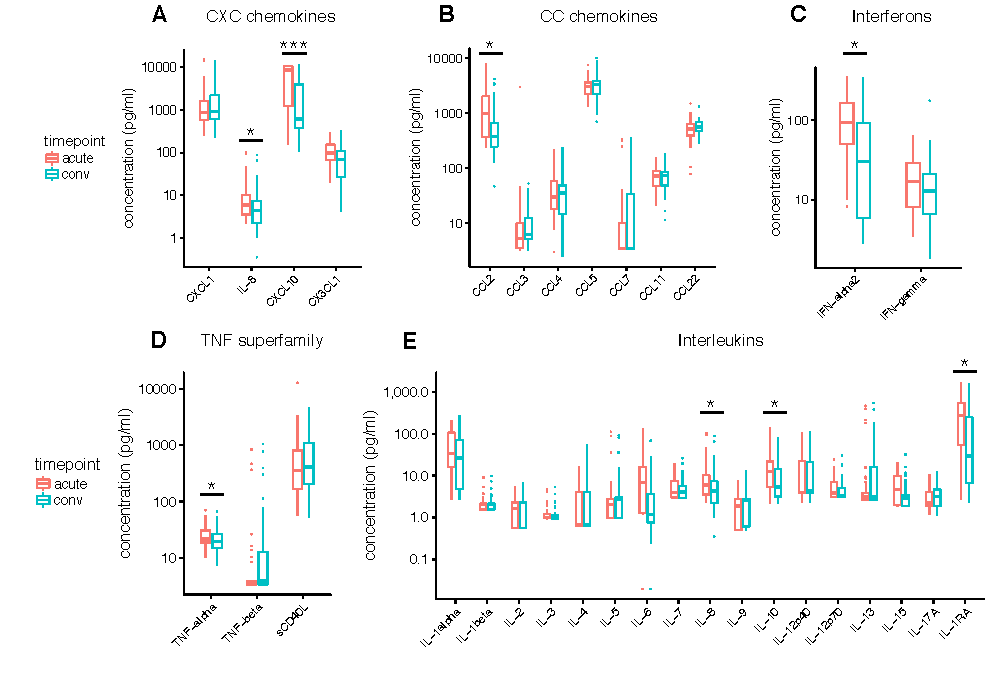
\includegraphics[width=\textwidth]{chap6/fig_5_luminex}
  \caption[Differences in serum cytokine and chemokine levels between the acute and convalescent phase samples]{
  \textbf{Differences in serum cytokine and chemokine levels between the acute and convalescent phase samples.} Wilcoxon signed-rank test was used to determine statistical significance, with a Benjamini-Hochberg adjustment for FDR (n = 41). *\emph{P} < 0.05, ***\emph{P} < 0.001. A, CXC chemokines. B, CC chemokines. C, interferons. D, TNF superfamily cytokines. E, interleukins. Note that IL-8 is both a CXC chemokine (CXCL8) and an interleukin, so it is depicted twice. Growth factors and colony-stimulating factors are shown in Appendix Figure \ref{fig:nonsig_luminex}.
  }
  \label{fig:luminex}
\end{figure*}

To profile the effect of CHIKV on circulatory markers for inflammation and immune signaling, we used a multiplexed microbead immunoassay (Luminex) to measure serum concentrations of 41 cytokines, chemokines, and growth factors in all 84 samples. In our study, seven cytokines were significantly different (Wilcoxon signed-rank test with Benjamini-Hochberg adjustment) across acute and convalescent timepoints at FDR < 0.05 (Figure \ref{fig:luminex}A-E). The strongest contrast was the IFN-γ inducible, monocyte-secreted chemokine CXCL10 (BF \emph{P} = 0.00085). Significant increases (FDR < 0.05) were also observed for IL-10 (a monocyte-secreted anti-inflammatory cytokine), CCL2 (monocyte chemoattractant protein 1), IFN-α2, TNF-α, IL-8, and IL-1RA. There were no significant differences observed among growth factors or colony-stimulating factors (Appendix Figure \ref{fig:nonsig_luminex}). No analyte concentrations were significantly decreased during acute infection.

To determine if cytokine levels could be associated with changes in specific cell \subcommunities{}, we correlated log-scaled Luminex analyte concentrations with log-scaled \subcommunity{} frequencies (using Pearson’s \emph{r}). Hierarchical clustering revealed that cytokine and growth factors concentrations tended to correlate with each other rather than with any of the subpopulation frequencies (Appendix Figure \ref{fig:corrplot_luminex_cytof_bothtimes}). This remained unchanged when stratifying into acute phase (Appendix Figure \ref{fig:corrplot_luminex_cytof_acute}) or convalescent phase (Appendix Figure \ref{fig:corrplot_luminex_cytof_conv}) samples, with the only exception being a cluster containing CXCL1, sCD40L, PDGF-AA, and PDGF-AB/BB that consistently separated from one major cluster containing all other Luminex analytes. Since the most pronounced expansions during the acute phase involved monocyte subpopulations, we then performed a more focused analysis on correlations between all cytokines and monocyte subpopulations, stratifying by timepoint to capture potential regulatory relationships rather than the primary contrast of the study. Within acute phase samples, cytokines generally had varied correlations with each of the monocyte subpopulations, but at the convalescent timepoint, the monocyte chemoattractant CCL2 clustered separately from all other cytokines and had positive correlations with all monocyte subpopulations (Figure \ref{fig:luminex_monocyte_corr}, BF \emph{P} = 0.0021). This is suggestive of a relatively important regulatory role for CCL2 on monocyte populations during the convalescent phase of infection.

\begin{figure*}[hb]
  \centering
  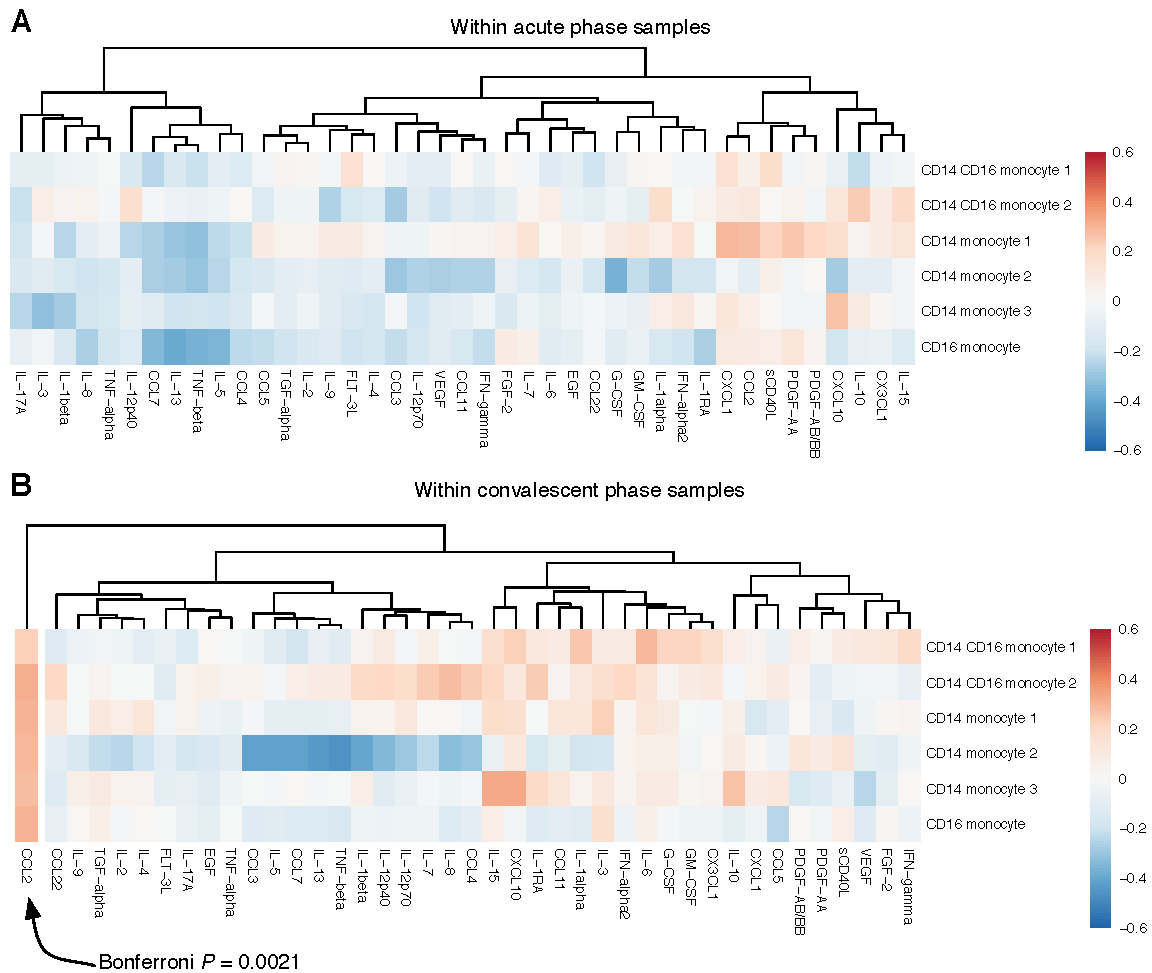
\includegraphics[width=\textwidth]{chap6/fig_S14_corrplots_cytokines_monocytes.pdf}
  \caption[Clustered heatmap of Pearson correlations between log-scaled serum cytokine concentration and log-scaled monocyte subphenotype frequencies]{
  \textbf{Clustered heatmap of Pearson correlations between log-scaled serum cytokine concentration and log-scaled monocyte subphenotype frequencies.} A, within acute phase samples. B, within convalescent phase samples.
  }
  \label{fig:luminex_monocyte_corr}
  \setfloatalignment{b}
\end{figure*}

\subsection{Acute infection associates with upregulated transcription of mo\-no\-cyte-associated cytokine genes}

To capture global transcriptional changes during CHIKV infection, polyadenylated RNA from whole blood was analyzed by RNA-seq for all 42 patients at both sampled timepoints with two technical replicates per sample. A Tuxedo pipeline was used for read alignment, quantification and differential expression analysis of genes. Since previous studies of gene and protein changes during acute CHIKV infection targeted cytokines, chemokines, and innate immunity mechanisms,\autocite{Chow2011,Hoarau2010,Ng2009,Teng2015,Wauquier2011} we first present results for differentially expressed genes in these pathways for comparison with our Luminex data and the literature, before moving to a global analysis in the subsequent section.

Appendix Figure \ref{fig:corrplot_luminex_mrna_both} shows that across the two timepoints, log-scaled serum concentrations for the significantly CHIK-upregulated cytokines (as measured by Luminex, Figure \ref{fig:luminex}) did not correlate with whole blood gene expression for corresponding genes, using log-scaled units of fragments per kilobase of exon per million reads mapped (FPKM). Since this could be due to different “baseline” serum cytokine or cytokine gene expression levels, we repeated the analysis with all acute phase measurements normalized against the convalescent phase measurements, but clustering did not change (Appendix Figure \ref{fig:corrplot_luminex_mrna_normacuteconv}). This suggests that the regulation of serum cytokine levels is not primarily driven by transcriptional changes in leukocytes, but could involve substantial expression from other tissues and secretory and protein-level regulatory processes. Alternatively, the technical variance of the Luminex assay for our samples may simply have been too high to draw out meaningful correlations with gene expression. 

\begin{sidewaysfigure}[hp]
  \sidewaysvspace
  \centering
  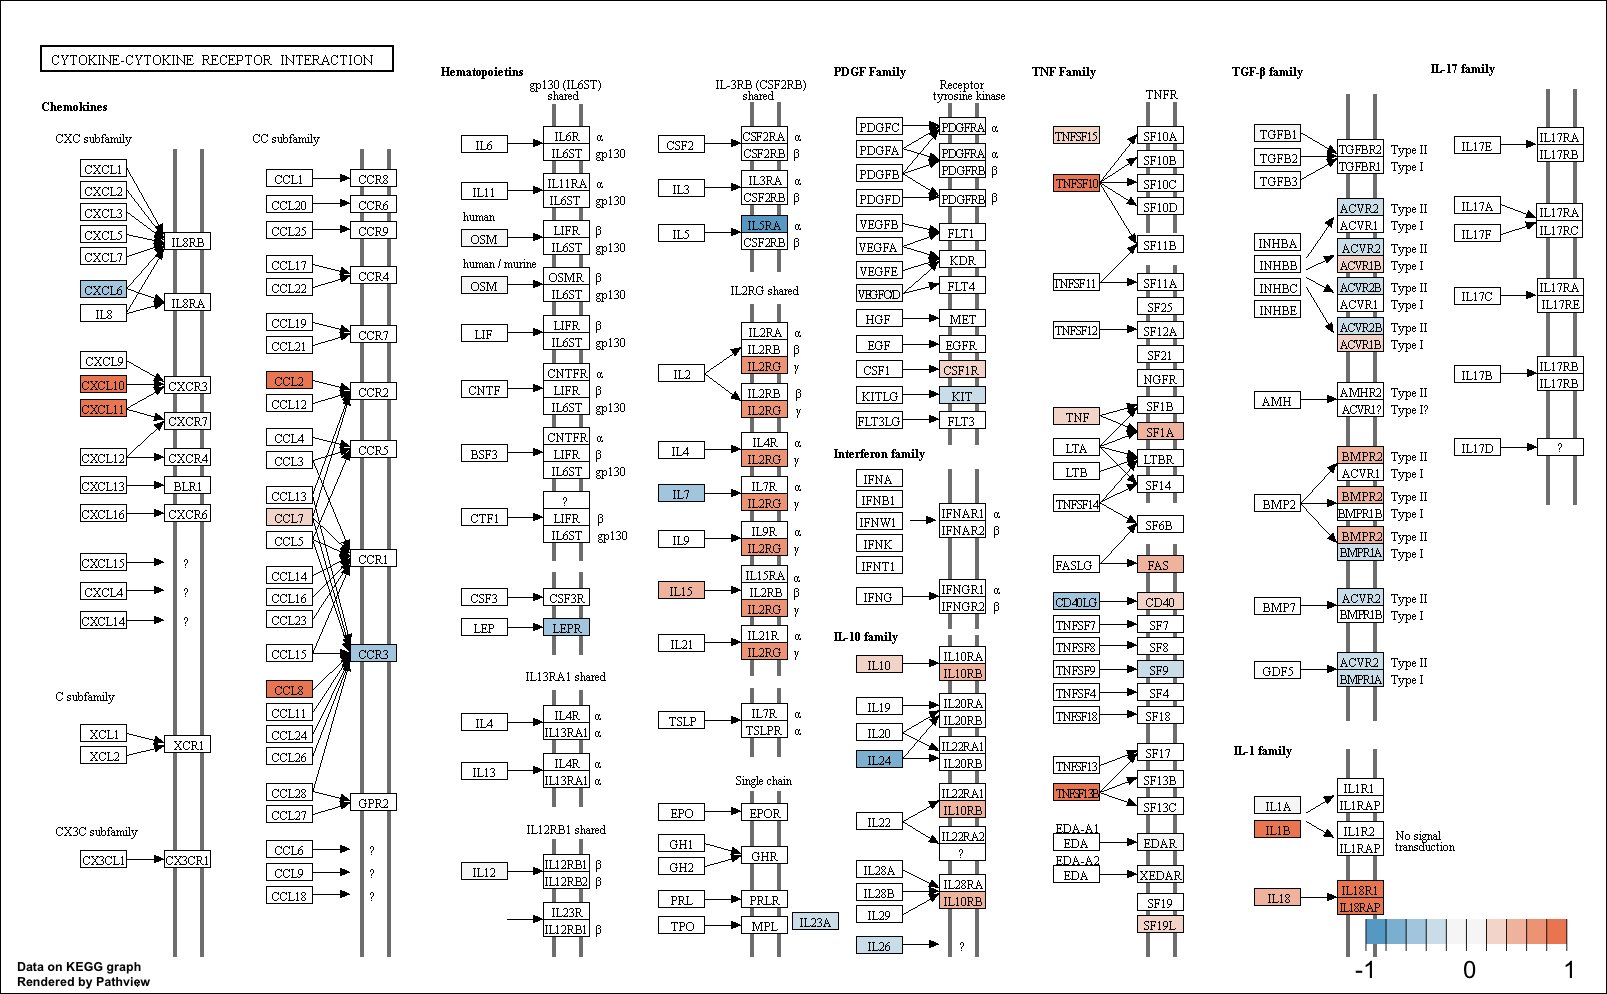
\includegraphics[width=\textwidth]{chap6/fig_S17_hsa04060.timepoint.log2fc.png}
  \fullwidthlabelcaption{fig:pathview_hsa04060}{Pathview plot of log\subs{2} fold change in expression of cytokine and receptor genes}{
  \textbf{Pathview plot of log\subs{2} fold change in gene expression between acute and convalescent timepoints for the cytokine-cytokine receptor interaction pathway}, using KEGG annotations (accession \href{http://www.genome.jp/dbget-bin/www\textunderscore bget?hsa04060}{hsa04060}). Positive values indicate upregulation during the acute phase of infection.
  }
\end{sidewaysfigure}

Differential expression of all genes was quantified by log\subs{2} fold change (log2FC) in units of FPKM and considered significant at an FDR threshold of <0.05. Among CXC and CC subfamily chemokines, we observed transcriptional upregulation of \emph{CXCL10}, \emph{CXCL11}, \emph{CCL2}, \emph{CCL7}, and \emph{CCL8} (Figure \ref{fig:pathview_hsa04060}). Of these, monocyte-secreted \emph{CXCL10} and monocyte chemoattractant \emph{CCL2} concur with the changes in serum cytokine concentrations described above (Figure \ref{fig:luminex}A-B), and \emph{CCL8} (whose gene product was not measured with Luminex) is notable for being another monocyte chemoattractant (MCP-2). Interestingly, although serum IFN-α levels were significantly elevated during acute infection (Figure \ref{fig:luminex}C), none of the interferon family genes were differentially expressed (Figure \ref{fig:pathview_hsa04060}). Upregulation of the \emph{TNF} gene is concordant with the significant increase in serum TNF-α concentration (Figures \ref{fig:pathview_hsa04060} and \ref{fig:luminex}D), and other significantly upregulated TNF superfamily genes included \emph{TNFSF15}, \emph{TNFSF10}, and \emph{TNFSF13B} (Figure \ref{fig:pathview_hsa04060}). While upregulation of \emph{IL10} gene expression was concordant with the serum cytokine measurements, in contrast to those data, we did not observe differential expression of \emph{IL8} (Figures \ref{fig:pathview_hsa04060} and \ref{fig:luminex}E). 

We also examined differential expression of genes during acute infection for known components of innate immunity pathways annotated in KEGG\autocite{Ogata1999} (Appendix Figures \ref{fig:pathview_hsa04062}-\ref{fig:pathview_hsa05164}). Of these pathways, JAK-STAT signaling genes were significantly transcriptionally upregulated, with smaller but significant upregulation of NF-κB genes (Appendix Figures \ref{fig:pathview_hsa04062} and \ref{fig:pathview_hsa04630}). Among toll-like receptor (TLR) genes, \emph{TLR5} and \emph{TLR3} (whose gene product is a dsRNA receptor) were significantly upregulated (Appendix Figure \ref{fig:pathview_hsa04620}). Both \emph{RIG-I} and \emph{MDA5}, which are cellular sensors for viral RNA, were significantly upregulated (Appendix Figure \ref{fig:pathview_hsa04622}). Of the TNF superfamily receptors, \emph{TNFR1} was upregulated but \emph{TNFR2} was not (Appendix Figure \ref{fig:pathview_hsa04668}). Of the interferon regulatory factor (IRF) genes annotated in KEGG, expression of \emph{IRF7} and \emph{IRF9} were significantly upregulated, and interestingly, all downstream transcriptional targets of IRF9 annotated in KEGG (\emph{MX1}, OAS genes, \emph{ADAR}, and \emph{PML}) were consistently upregulated during acute infection (Appendix Figure \ref{fig:pathview_hsa05164}). (Fold change values for all quantified genes and \emph{q} values are provided in Supplementary Data S2.) In general, our observed modulations of human innate immunity pathways were comparable to differentially expressed genes reported for a mouse model in a recent study\sidecite[-7.2cm]{Wilson2017} (see Discussion). 

\subsection{Transcriptomic signatures for acute infection, severity, viral titer, and immunogenicity}

RNA-seq enables the estimation of transcript abundances and transcript-level differential expression analyses that may offer insights not available from gene-level quantification.\sidecite[-9.5cm]{Anders2012,Trapnell2013} We performed pseudoalignment-based quantification of transcript abundances in units of transcripts per million (TPM), followed by differential expression analysis.
\begin{marginfigure}[-7.5cm]
  \centering
  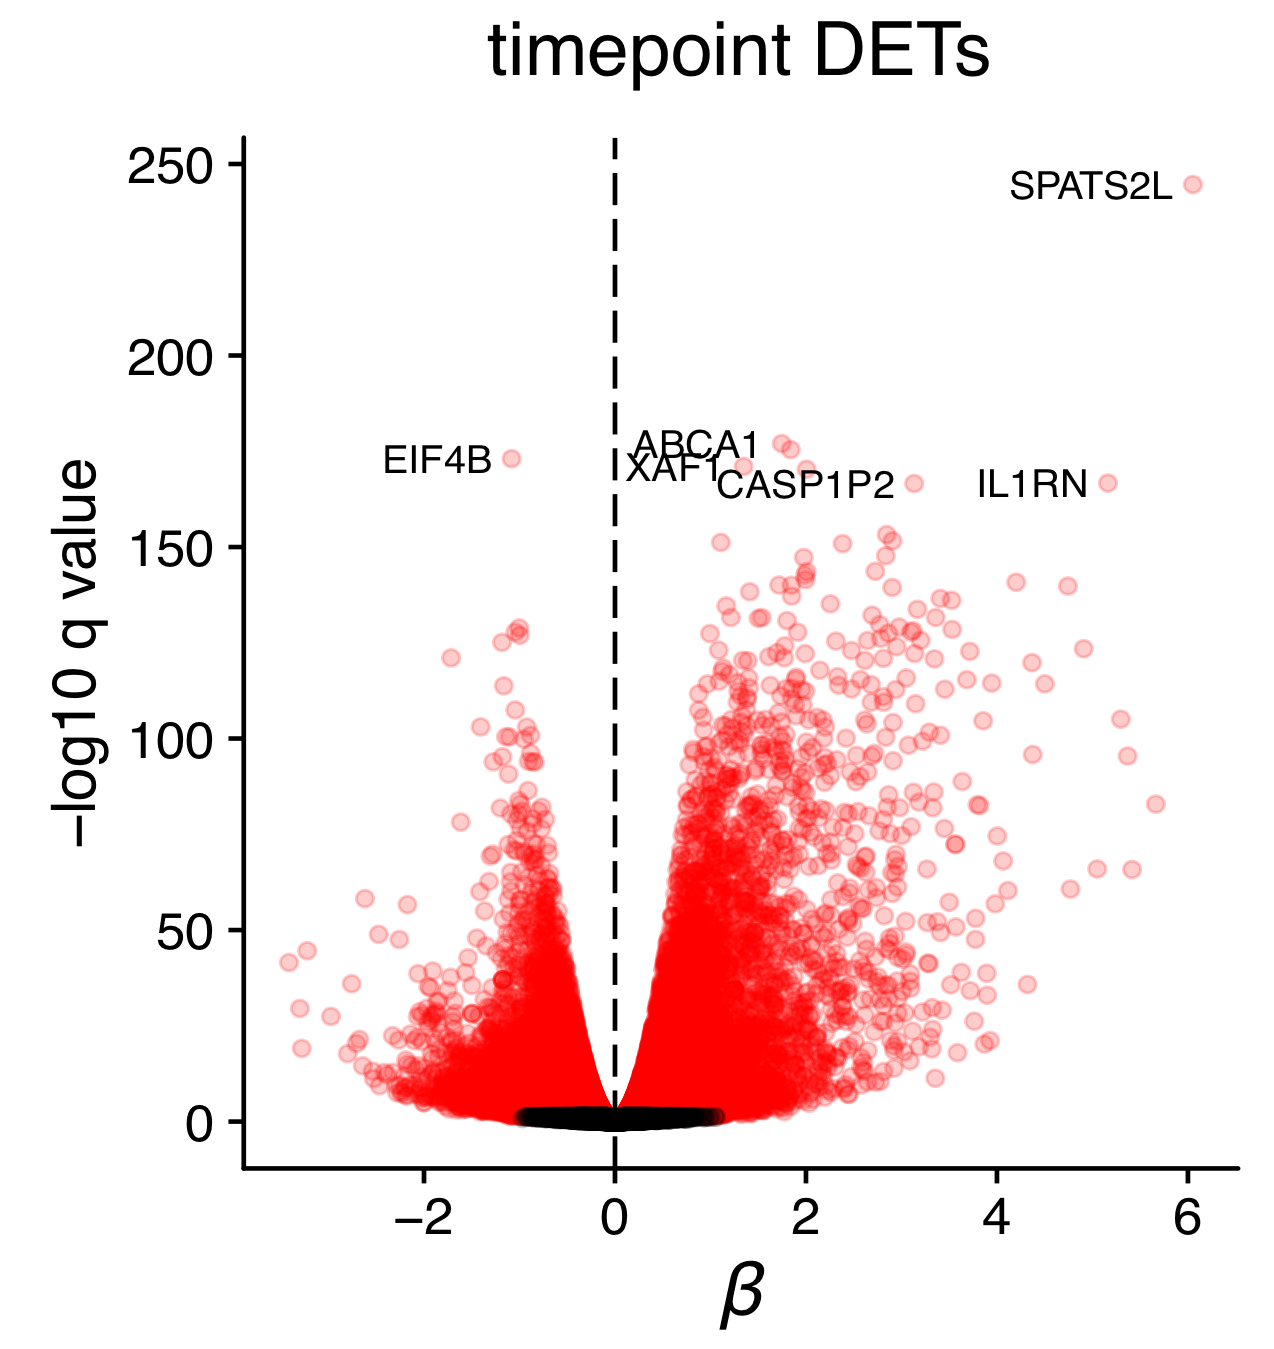
\includegraphics[width=\textwidth]{chap6/fig_6a_DET_timepoint_volcano}
  \caption[Volcano plot of differentially expressed host transcripts between acute and convalescent phase samples]{
  \textbf{Volcano plot of differentially expressed host transcripts between acute and convalescent phase samples}, with negative log\subs{10} scaled \emph{q} values (Benjamini-Hochberg adjusted \emph{P} values) on the Y axis, and the modeled $\beta$ coefficient for each transcript (corresponding to natural log transformed effect sizes) on the X axis. Transcripts to the right of the vertical dashed line were comparatively upregulated in acute phase samples, while transcripts to the left were upregulated during the convalescent phase. Transcripts that pass FDR < 0.05 are colored red. Top transcripts by \emph{q} value are individually labeled by their corresponding gene symbol. 
  }
  \label{fig:DET_timepoint_volcano}
\end{marginfigure}
\begin{figure*}[hp]
  \centering
  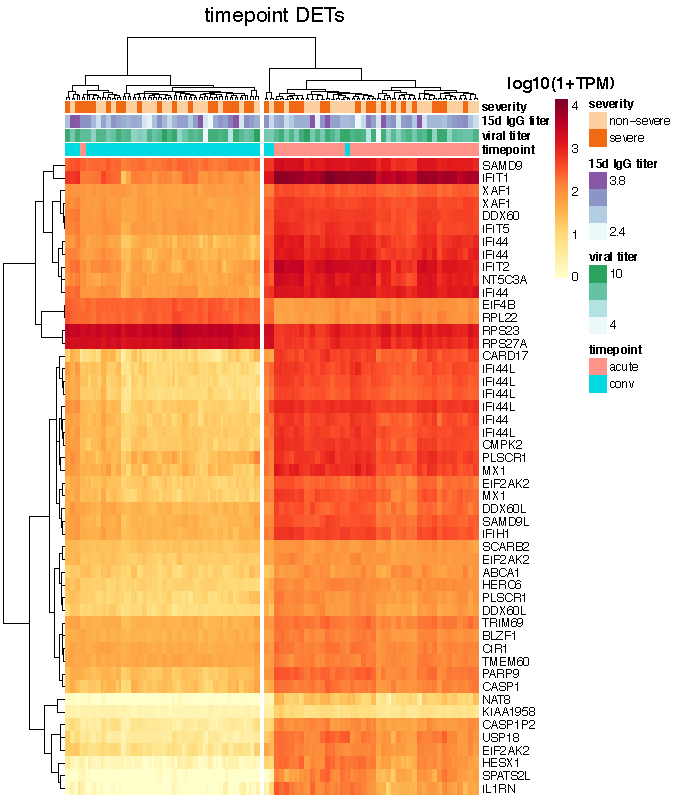
\includegraphics[width=0.85\textwidth]{chap6/fig_6b_DET_timepoint_heatmap}
  \fullwidthlabelcaption{fig:DET_timepoint_heatmap}{Top 50 differentially expressed host transcripts for CHIKV infection phase}{
  \textbf{Top 50 differentially expressed host transcripts for CHIKV infection phase.} Heatmap of expression measured in log\subs{10} scaled 1 + transcripts per million (TPM) for top 50 differentially expressed transcripts between acute and convalescent phase samples (2 technical replicates per patient sample). Clinical variables are depicted for all samples across the top of the heatmap; 15d post symptom onset immunoglobulin G (IgG) titer and viral titer (which was measured during the acute phase) are both in units of log\subs{10} dilutions. Hierarchical clustering (using complete linkage) was applied to both samples (X axis) and transcripts (Y axis). Two major clusters of samples (largely separating acute and convalescent samples) are highlighted.
  }
\end{figure*}
After adjusting for age and gender covariates, a strong transcriptional signature for timepoint (acute vs.\ convalescent) emerged (Figure \ref{fig:DET_timepoint_volcano}), with 28,015 transcripts differentially expressed at FDR < 0.05. The top differentially expressed transcripts (DETs), ordered by \emph{P} value, were products of the \emph{SPATS2L}, \emph{IL1RN}, \emph{EIF4B}, \emph{ABCA1}, \emph{XAF1}, and \emph{CASP1P2} genes. Hierarchical clustering of the samples by quantification of the top 50 differentially expressed transcripts readily separated samples by timepoint, with only 8/160 (5\%) of samples misclassified between the two major clusters (Figure \ref{fig:DET_timepoint_heatmap}). All paired technical replicates clustered together. The top 50 DETs notably contained many interferon-induced (IFI prefix) gene products that cluster along the vertical axis (Figure \ref{fig:DET_timepoint_heatmap}).

\begin{marginfigure}[-3cm]
  \centering
  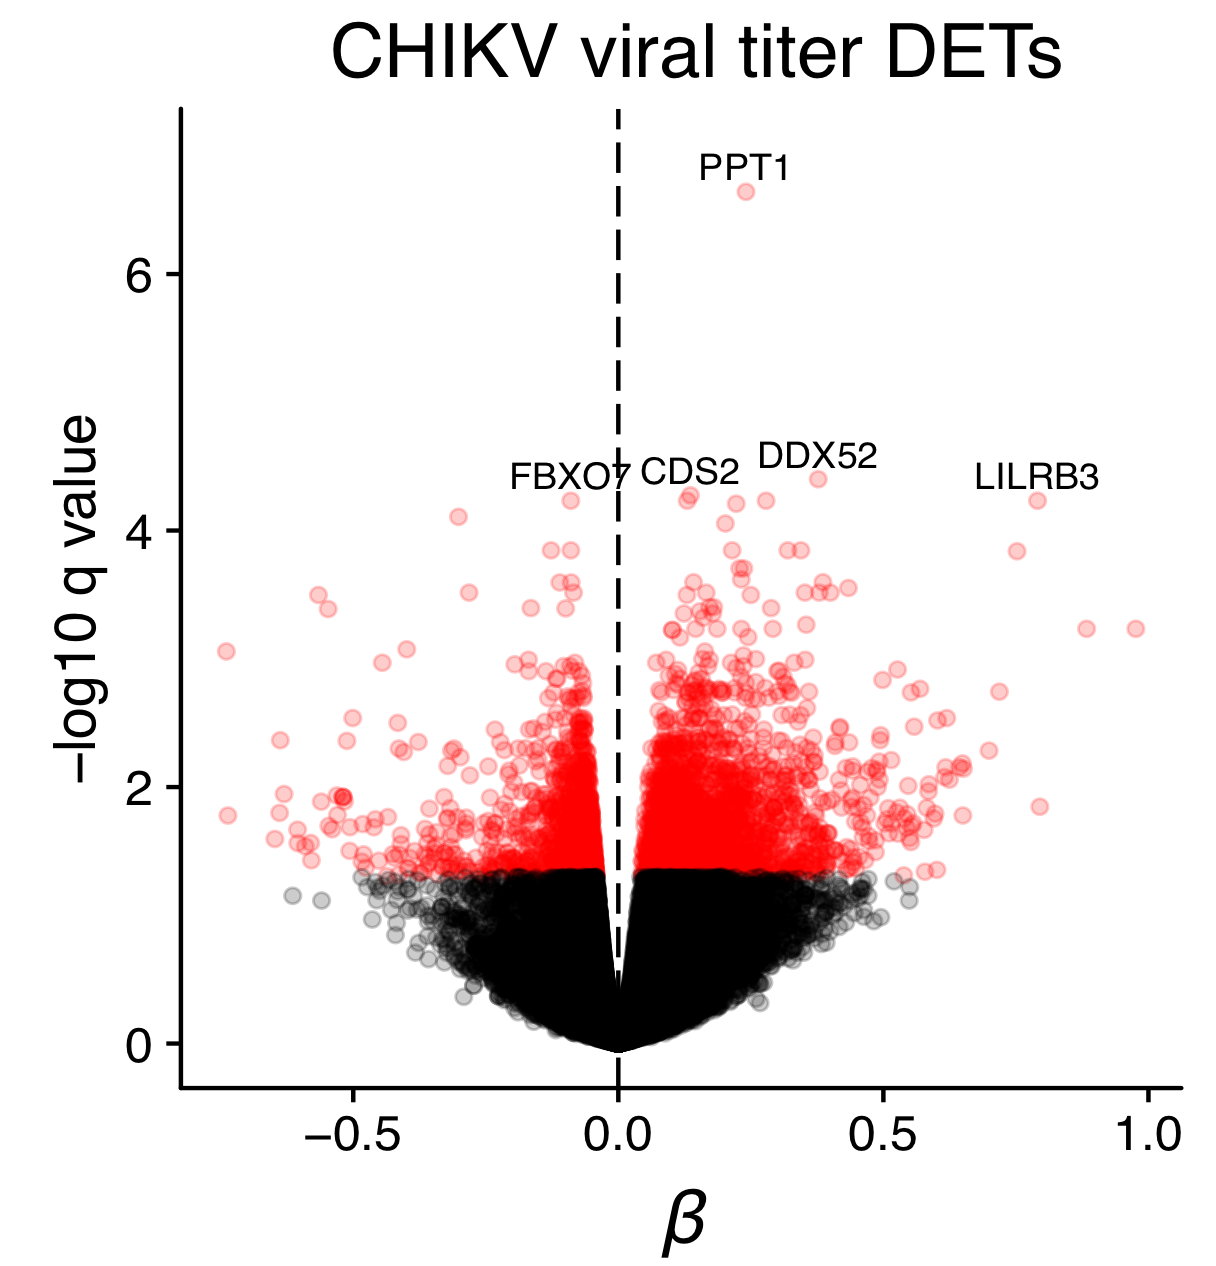
\includegraphics[width=\textwidth]{chap6/fig_6c_DET_viral_volcano}
  \caption[Volcano plot of differentially expressed host transcripts for viremic load]{
  \textbf{Volcano plot} as in Figure \ref{fig:DET_timepoint_volcano} but for DETs between samples with higher and lower CHIKV viral titer. Transcripts to the right of the vertical dashed line associated with higher viral titer, while transcripts to the left associated with lower viral titer. 
  }
  \label{fig:DET_viral_volcano}
\end{marginfigure}

Adding the log-scaled acute phase CHIK viral titer as a variable to the model of transcript expression produced a separate and substantial signature for transcription correlating with viral titer (Figure \ref{fig:DET_viral_volcano}), with 3,326 DETs at FDR < 0.05. In Figure \ref{fig:DET_viral_volcano}, an increase in transcription corresponding to higher viral titers were modeled as a positive fixed effect coefficient $\beta$. Top DETs for viral titer (by \emph{P} value) were products of the \emph{PPT1}, \emph{DDX52}, \emph{LILRB3}, \emph{CDS2}, and \emph{FBXO7} genes, with all but the last upregulated in cases with higher viremia.

We assessed the composition of these two large signatures with standard gene set enrichment analyses for functional annotation libraries. The top 1,000 genes in the timepoint DET signature were most significantly enriched for gene ontology (GO), Panther, and Reactome annotations related to defense against viral infection, TLR signaling, and interferon signaling (Table \ref{tab:chik_det_enrichr}). The top 1,000 genes in the viral titer DET signature were most significantly enriched for terms related to leukocyte activation, chemokine and cytokine signaling, and interferon signaling (Table \ref{tab:chik_det_enrichr}). These enrichments suggest that the timepoint of infection sensibly corresponds to a maximal contrast in transcription of innate antiviral immunity genes, while the level of viremia correlates with increased transcription of immune cell activation and recruitment signals.

\begin{marginfigure}[-9.5cm]
  \centering
  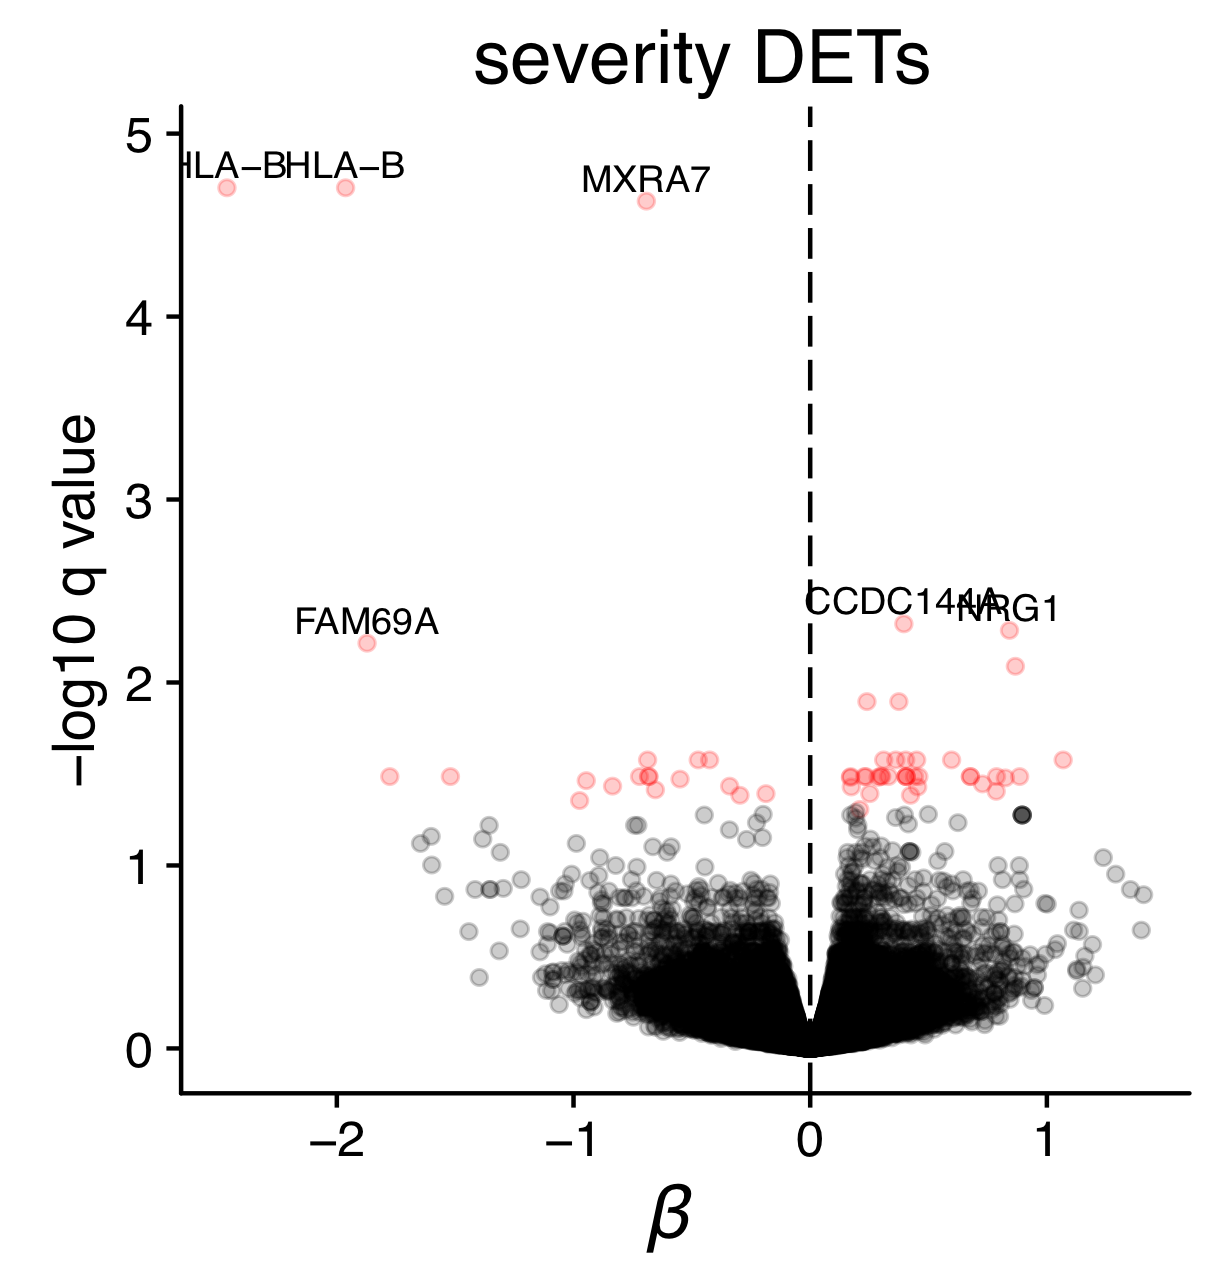
\includegraphics[width=\textwidth]{chap6/fig_6d_DET_severity_volcano}
  \caption[Volcano plot of differentially expressed host transcripts for symptom severity]{
  \textbf{Volcano plot} as in Figure \ref{fig:DET_timepoint_volcano} but for DETs between patients with more severe and less severe acute phase symptoms. Transcripts to the right of the vertical dashed line were comparatively upregulated in severe cases, while transcripts to the left were upregulated in non-severe cases. 
  }
  \label{fig:DET_severity_volcano}
\end{marginfigure}
\begin{marginfigure}[-1cm]
  \centering
  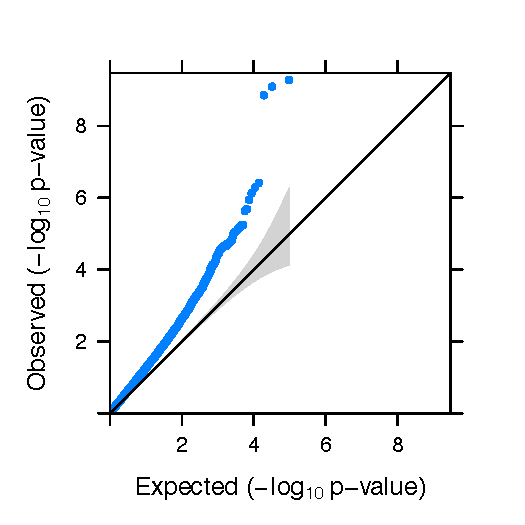
\includegraphics[width=0.8\textwidth]{chap6/fig_S24_sleuth-wt-severity-qq}
  \caption[Q-Q plot of the distribution of observed –log\subs{10} \emph{P} values for severity DETs against the distribution expected under the null hypothesis]{
    \textbf{Q-Q plot of the distribution of observed –log\subs{10} \emph{P} values for severity DETs against the distribution expected under the null hypothesis.} Gray shaded band indicates the 95\% confidence interval for the null distribution.
  }
  \label{fig:DET_severity_qq}
\end{marginfigure}
\begin{table*}[htb]
  \centering
\footnotesize
\begin{tabular}{P{0.85in} P{0.75in} P{1.65in} l l l P{0.7in}}
  \toprule
  Gene set$^a$ (\#~genes) & Annotation set & Term & Overlap & \emph{q} value$^b$ & \emph{Z}-score & Combined score$^c$ \\
  \midrule
  \multirow{9}{0.85in}{Top 1000 DETs for timepoint: acute vs. convalescent (593)}
   & \multirow{3}{0.75in}{GO Biological Process 2015} & defense response to virus  & 40/147 & 5.98e-24 & -2.26 & 120 \\
     \cmidrule{3-7}
   &  & response to virus  & 47/250 & 1.50e-21 & -2.37 & 114 \\
     \cmidrule{3-7}
   &  & viral life cycle  & 36/118 & 1.51e-23 & -2.14 & 112 \\
   \cmidrule{2-7}
   & \multirow{3}{0.75in}{Panther 2016} & toll receptor signaling pathway & 7/49 & 0.0425 & -1.51 & 4.76 \\
     \cmidrule{3-7}
   &  & apoptosis signaling pathway & 8/102 & 0.191 & -1.39 & 2.30 \\
     \cmidrule{3-7}
   &  & oxidative stress response & 4/24 & 0.190 & -1.31 & 2.18 \\
   \cmidrule{2-7}
   & \multirow{3}{0.75in}{Reactome 2016} & interferon signaling & 45/196 & 2.41e-24 & -2.10 & 114 \\
     \cmidrule{3-7}
   &  & eukaryotic translation elongation & 32/89 & 7.89e-24 & -2.01 & 107 \\
     \cmidrule{3-7}
   &  & L13a-mediated translational silencing of ceruloplasmin expression & 34/106 & 7.89e-24 & -1.95 & 103 \\
  \cmidrule{1-7}
  \multirow{9}{0.85in}{Top 1000 DETs for viral titer (874)}
   & \multirow{3}{0.75in}{GO Biological Process 2015} & leukocyte activation  & 47/373 & 2.50e-07 & -2.38 & 36.2 \\
     \cmidrule{3-7}
   &  & cellular response to cytokine stimulus  & 50/471 & 8.20e-06 & -2.46 & 28.8 \\
     \cmidrule{3-7}
   &  & cytokine-mediated signaling pathway & 41/342 & 8.20e-06 & -2.39 & 28.0 \\
   \cmidrule{2-7}
   & \multirow{3}{0.75in}{Panther 2016} & Inflammation mediated by chemokine and cytokine signaling pathway & 23/188 & 0.000695 & -1.83 & 13.3 \\
     \cmidrule{3-7}
   &  & CCKR signaling map & 17/165 & 0.0346 & -1.71 & 5.77 \\
     \cmidrule{3-7}
   &  & T cell activation & 10/73 & 0.0346 & -1.40 & 4.71 \\
   \cmidrule{2-7}
   & \multirow{3}{0.75in}{Reactome 2016} & Immune System & 111/1547 & 0.000136 & -2.23 & 19.9 \\
     \cmidrule{3-7}
   &  & Interferon Signaling & 26/196 & 0.000253 & -2.09 & 17.4 \\
     \cmidrule{3-7}
   &  & Cytokine Signaling in Immune system & 51/620 & 0.00427 & -2.39 & 13.0 \\
  \bottomrule
\end{tabular}
  \caption[Gene set enrichment analysis of DET signatures][0.5cm]{\textbf{Gene set enrichment analysis of DET signatures.}
  Abbreviations: DET, differentially expressed transcript; GO, gene ontology; CCKR, cholecystekinin receptor.
  \captionfootnotetext{a}{Gene sets were constructed by taking the top 1,000 DETs in each category, ordered by ascending \emph{q} value, and mapping to unique gene symbols}
  \captionfootnotetext{b}{\emph{q} values are \emph{P}-values adjusted using the Benjamini-Hochberg method.}
  \captionfootnotetext{c}{Combined scores are the product of negative log \emph{P}-values and the \emph{Z}-score as in \textcite{Chen2013}; the top three terms per annotation set, ordered by combined score, are displayed in this table.}
}
  \label{tab:chik_det_enrichr}
\end{table*}

Although the phase of infection and the level of viremia were expected to produce strong transcriptional signatures, we sought potential signatures for downstream clinical outcomes, such as the severity of acute phase symptoms or the CHIKV IgG titer measured at 15d p.s.o., a correlate for humoral immunogenicity. For symptom severity, adding the severe vs.\ non-severe categorization of cases to the model produced a small differential expression signature of 56 transcripts at FDR < 0.05 (Figure \ref{fig:DET_severity_volcano}), with \emph{P} values for the top three transcripts displaying divergence from the remaining distribution (Figures \ref{fig:DET_severity_volcano} and \ref{fig:DET_severity_qq}). Two of these transcripts were from \emph{HLA-B}, one of which is its canonical protein-coding transcript, and the other of which is a retained intron; the third is the canonical transcript of \emph{MXRA7}, which encodes a poorly characterized single-pass membrane protein. Hierarchical clustering of samples by TPM for the top 10 DETs revealed that one of the four major clusters associates with 63/80 (79\%) of samples from severe cases, and the \emph{HLA-B} transcripts strongly associate with exactly two of the three remaining clusters (Figure \ref{fig:DET_timepoint_heatmap}).
\begin{figure*}[htb]
  \centering
  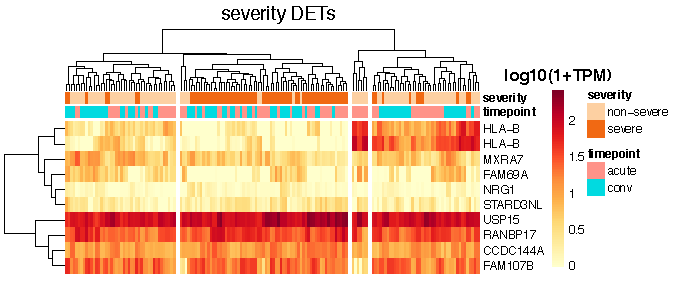
\includegraphics[width=0.85\textwidth]{chap6/fig_6e_DET_severity_heatmap}
  \caption[Top 10 differentially expressed host transcripts for CHIKV symptom severity]{
  \textbf{Heatmap of DET expression} as in Figure \ref{fig:DET_timepoint_heatmap} but for the top 10 DETs between samples from severe and non-severe cases. Four major clusters of samples are highlighted.
  }
  \label{fig:DET_severity_heatmap}
\end{figure*}
Overexpression of these three transcripts in non-severe cases was consistent across both timepoints (Figure \ref{fig:DET_severity_boxplot}), and of the three next highly ranked transcripts, two were associated with severe cases (\emph{CCDC144A}, \emph{NRG1}) while one was associated with non-severe cases (\emph{FAM69A}).

\begin{figure}[htb]
  \centering
  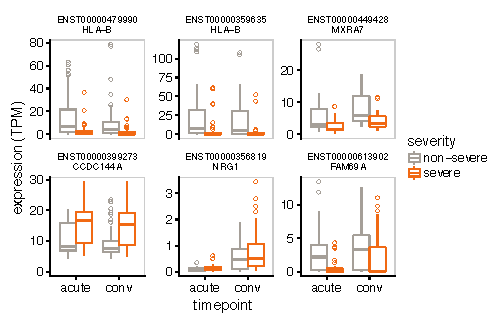
\includegraphics[width=\textwidth]{chap6/fig_6f_DET_severity_boxplot}
  \caption[Differential expression of severity DETs holds across both timepoints][2cm]{
  \textbf{Expression of six top DETs} (ranked by \emph{q} value) between samples from severe (orange) and non-severe (gray) cases. Expression is measured in TPM. Differences in expression appear to be independent of sample timepoint (X axis). 
  }
  \label{fig:DET_severity_boxplot}
\end{figure}

\begin{marginfigure}[-3.5cm]
  \centering
  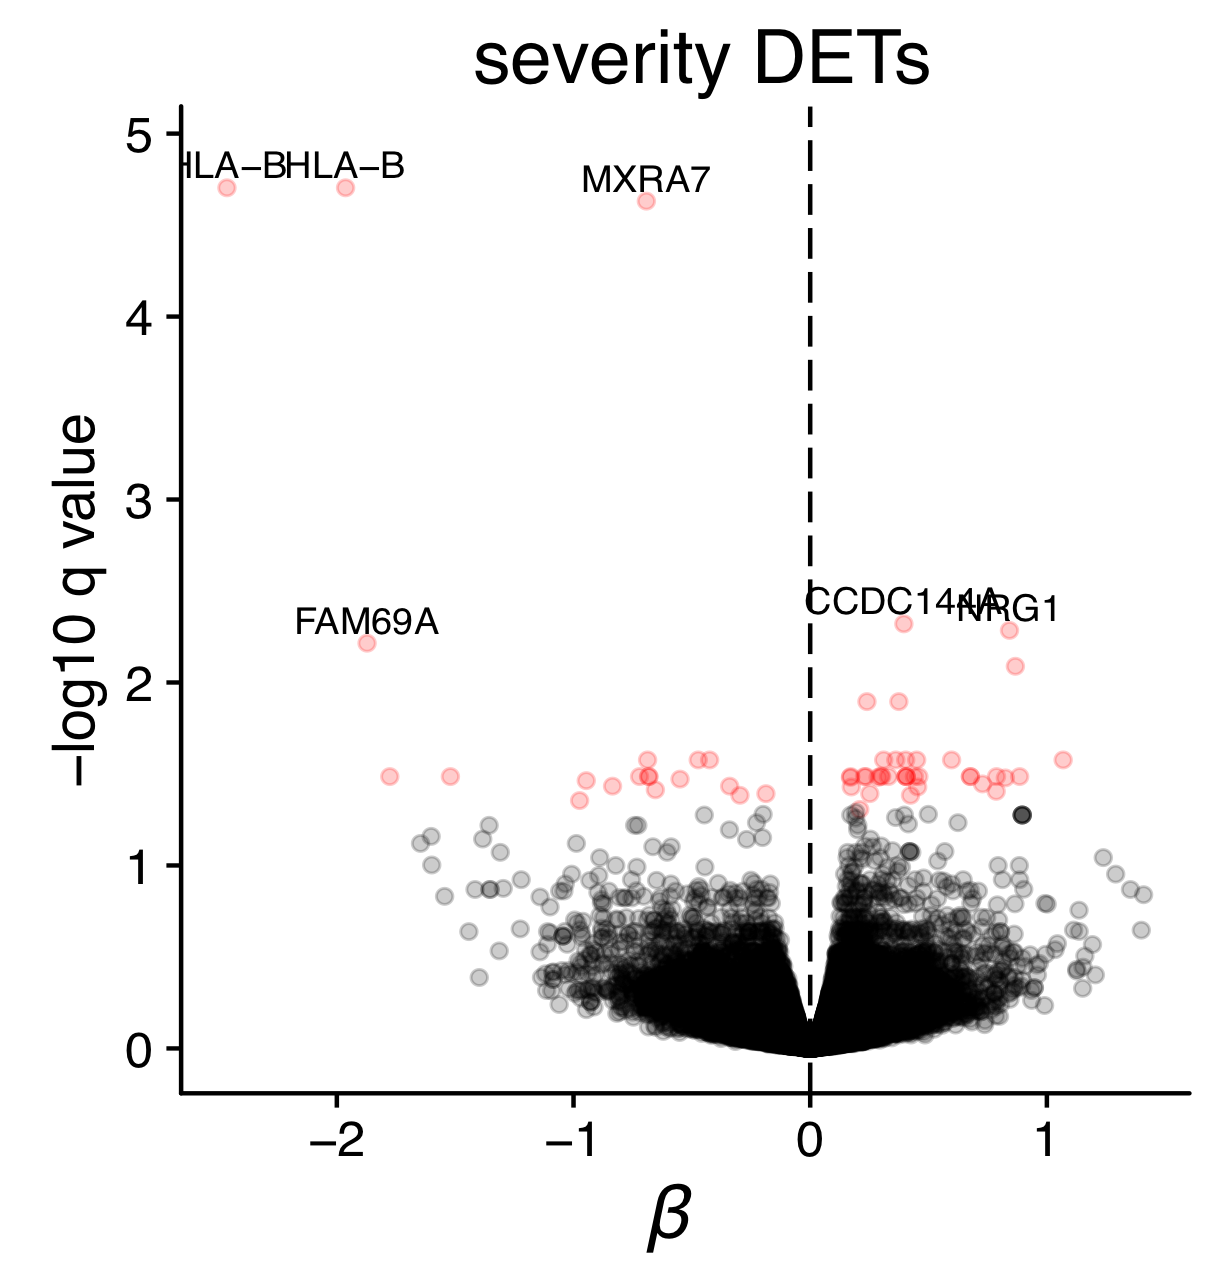
\includegraphics[width=\textwidth]{chap6/fig_6d_DET_severity_volcano}
  \caption[Volcano plot of differentially expressed host transcripts for symptom severity]{
  \textbf{Volcano plot} as in Figure \ref{fig:DET_timepoint_volcano} but for DETs between patients with higher and lower 15d post symptom onset CHIKV IgG titers. Transcripts to the right of the vertical dashed line were comparatively upregulated in patients with a higher 15d IgG, while transcripts to the left were upregulated in patients with lower 15d IgG.
  }
  \label{fig:DET_IgG_volcano}
\end{marginfigure}

We found a similarly sized signature for the 15d p.s.o. CHIKV IgG titer, with 63 DETs at FDR < 0.05 (Figure \ref{fig:DET_IgG_volcano}). Top-ranked transcripts by \emph{P} value were again notable for including HLA genes, such as two transcripts of \emph{HLA-A} and two transcripts of \emph{HLA-DOB} among the top eight transcripts.

Complete tables of all DETs, $\beta$ values, and \emph{q} values for the timepoint, viral titer, symptom severity, and IgG titer contrasts are provided as Supplementary Data S3, S4, S5, and S6, respectively.

\subsection{Multiscale network analysis}

\begin{figure}[htb]
  \centering
  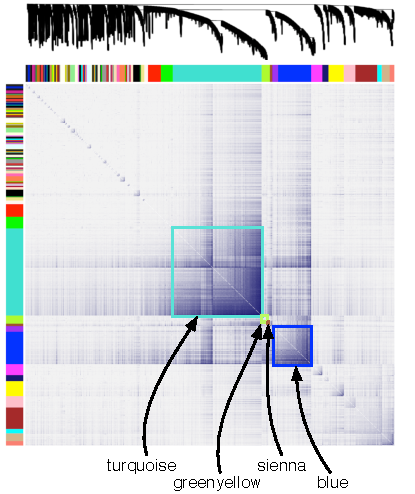
\includegraphics[width=\textwidth]{chap6/fig_7a_TOM}
  \caption[Topological overlap matrix (TOM) plot of coexpression network]{
  \textbf{Topological overlap matrix (TOM) plot of coexpression network} created from gene expression profiling of all 84 samples across both timepoints. At top, dendrogram of the hierarchical clustering of the matrix that undergoes a dynamic tree-cut operation to form 92 gene coxpression network modules (coEMs), depicted by the colored bars on the edges of the TOM plot (color assignment is arbitrary). Four coEMs are highlighted (boxes).
  }
  \label{fig:chik_TOM}
\end{figure}

To relate CHIKV-associated transcriptomic changes to changes in cell \subcommunity{} frequencies, serum cytokine concentrations, and clinical variables, we identified coexpression patterns among sets of genes to create coexpression network modules (coEMs) using whole genome coexpression network analysis (WGCNA).\autocite{Zhang2005} The coEMs could then be correlated with other variables to capture the genomic coregulatory structure from biological variability present across and within the timepoints. We identified 92 coEMs, which were named after arbitrary colors (Figures \ref{fig:chik_TOM} and \ref{fig:coEM_overlaps}). 
\begin{figure*}
  \centering
  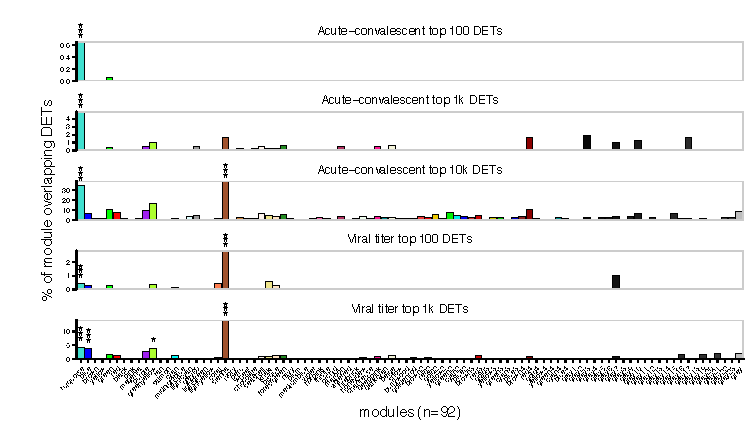
\includegraphics[width=\textwidth]{chap6/fig_7b_coEM_overlaps}
  \caption[Enrichment of five subsets of the DET signatures in the coexpression modules]{
  \textbf{Enrichment of five subsets of the DET signatures for CHIKV infection phase and viral titer} (see Figures \ref{fig:DET_timepoint_volcano} and \ref{fig:DET_viral_volcano}) among each of the 92 coEMs (X axis), showing the fractional overlap of the module with the DET signature (Y axis). *\emph{q} < 0.05, ***\emph{q} < 0.001; \emph{q} values are Benjamini-Hochberg adjusted \emph{P} values (Appendix Figure \ref{fig:coem_det_overlap_qvals} shows \emph{q} values for all tests). The four coEMs highlighted in Figure \ref{fig:chik_TOM} have at least one significant DET signature enrichment.
  }
  \label{fig:coEM_overlaps}
\end{figure*}
At a threshold of FDR < 0.05, four of these coEMs were significantly enriched for at least one of five gene sets derived from the previously acquired DET signatures for timepoint and viral titer (Figure \ref{fig:coEM_overlaps}). Of these enrichments, the most consistent and significant were turquoise (5/5 sets; max BF \emph{P} = 8.0e-07) and sienna (3/5 sets; max BF \emph{P} = 1.8e-08). DET enrichment \emph{q} values are depicted in Appendix Figure \ref{fig:coem_det_overlap_qvals}.

To explore the coregulatory structure between coEMs and clinical variables, we correlated each coEM eigengene (which is the first principal component of the expression of genes in the module) against all other coEM eigengenes and the clinical variables (Figure \ref{fig:coEM_corr}). This revealed that the turquoise module was strongly positively correlated with the convalescent phase (Pearson’s \emph{r} = 0.82), while the sienna module was strongly positively correlated with the greenyellow module (\emph{r} = 0.97) and negatively correlated with the convalescent phase (\emph{r} = -0.39) and turquoise module (\emph{r} = -0.40). The blue module was only weakly positively correlated with the turquoise module (\emph{r} = 0.37) and the convalescent phase (\emph{r} = 0.26). This suggests that in our study, the sienna module is most representative of acute-associated genes, while the turquoise module is most representative of convalescent-associated genes.

\begin{table*}[p]
  \centering
\footnotesize
\begin{tabular}{P{0.85in} P{0.75in} P{1.5in} l l l P{0.75in}}
  \toprule
  Gene set$^a$ (\#~genes) & Annotation set & Term & Overlap & \emph{q} value$^b$ & \emph{Z}-score & Combined score$^c$ \\
  \midrule
  \multirow{9}{0.85in}{sienna (370)}
   & \multirow{3}{0.75in}{GO Biological Process 2015} & regulation of cytokine production  & 28/482 & 0.000268 & -2.51 & 20.7 \\
     \cmidrule{3-7}
   &  & positive regulation of cytokine production  & 22/327 & 0.000279 & -2.45 & 20.1 \\
     \cmidrule{3-7}
   &  & regulation of immune effector process  & 18/264 & 0.00106 & -2.46 & 16.9 \\
   \cmidrule{2-7}
   
   & \multirow{3}{0.75in}{Reactome 2016} & immune system & 65/1547 & 1.81e-07 & -2.23 & 34.7 \\
     \cmidrule{3-7}
   &  & cytokine signaling in immune system & 26/620 & 0.0211 & -2.39 & 9.21 \\
     \cmidrule{3-7}
   &  & hemostasis & 23/552 & 0.0340 & -2.12 & 7.16 \\
   \cmidrule{2-7}
   
   & \multirow{3}{0.75in}{WikiPathways 2016} & type II interferon signaling & 6/37 & 5.35e-05 & -1.82 & 10.4 \\
     \cmidrule{3-7}
   &  & BDNF signaling pathway & 9/144 & 0.00141 & -1.92 & 6.84 \\
     \cmidrule{3-7}
   &  & senescence and autophagy in cancer & 8/105 & 0.000720 & -1.77 & 6.72 \\
  \cmidrule{1-7}
   
  \multirow{9}{0.85in}{blue (3,554)}
   & \multirow{3}{0.75in}{GO Biological Process 2015} & gene expression & 189/672 & 5.28e-08 & -2.34 & 39.2 \\
     \cmidrule{3-7}
   &  & hexose metabolic process & 67/187 & 6.37e-06 & -2.32 & 27.8 \\
     \cmidrule{3-7}
   &  & generation of precursor metabolites and energy & 107/375 & 0.000123 & -2.37 & 21.3 \\
   \cmidrule{2-7}
   
   & \multirow{3}{0.75in}{Reactome 2016} & infectious disease & 111/348 & 3.99e-08 & -2.39 & 40.7 \\
     \cmidrule{3-7}
   &  & HIV Infection & 80/222 & 3.91e-08 & -2.38 & 40.5 \\
     \cmidrule{3-7}
   &  & metabolism & 446/1908 & 3.91e-08 & -2.25 & 38.3 \\
   \cmidrule{2-7}
   
   & \multirow{3}{0.75in}{WikiPathways 2016} & proteasome degradation & 29/62 & 2.84e-05 & -1.91 & 20.0 \\
     \cmidrule{3-7}
   &  & B cell receptor signaling pathway & 33/97 & 0.00455 & -1.90 & 10.3 \\
     \cmidrule{3-7}
   &  & pathogenic \emph{E. coli} infection & 22/55 & 0.00455 & -1.74 & 9.40 \\
  \cmidrule{1-7}
  
  \multirow{9}{0.85in}{greenyellow (507)}
   & \multirow{3}{0.75in}{GO Biological Process 2015} & negative regulation of smooth muscle cell migration  & 4/12 & 0.223 & -2.65 & 3.97 \\
     \cmidrule{3-7}
   &  & regulation of smooth muscle cell migration  & 6/31 & 0.223 & -2.51 & 3.76 \\
     \cmidrule{3-7}
   &  & endosome to lysosome transport  & 5/31 & 0.662 & -2.61 & 1.08 \\
   \cmidrule{2-7}
   
   & \multirow{3}{0.75in}{Reactome 2016} & TNF signaling & 5/41 & 0.459 & -2.08 & 1.62 \\
     \cmidrule{3-7}
   &  & deposition of new CENPA-containing nucleosomes at the centromere & 5/52 & 0.459 & -2.04 & 1.59 \\
     \cmidrule{3-7}
   &  & nucleosome assembly & 5/52 & 0.459 & -2.03 & 1.58 \\
   \cmidrule{2-7}
   
   & \multirow{3}{0.75in}{WikiPathways 2016} & apoptosis modulation and signaling & 8/93 & 0.353 & -2.09 & 2.18 \\
     \cmidrule{3-7}
   &  & complement and coagulation cascades & 6/59 & 0.353 & -1.90 & 1.98 \\
     \cmidrule{3-7}
   &  & apoptosis modulation by HSP70 & 3/19 & 0.412 & -1.49 & 1.32 \\
  \bottomrule
\end{tabular}
  \fullwidthlabelcaption{tab:chik_coEM_enrichr}{Gene set enrichment analysis of coexpression modules.}{
  \textbf{Gene set enrichment analysis of coexpression modules.} Abbreviations: GO, gene ontology; BDNF, brain-derived neurotrophic factor; HIV, human immunodeficiency virus; TNF, tumor necrosis factor; CENPA, centromere protein A; HSP70, 70 kilodalton heat shock protein.
  \captionfootnotetext{a}{Number of unique gene symbols}
  \captionfootnotetext{b}{$\emph{q}$ values are \emph{P}-values adjusted using the Benjamini-Hochberg method.}
  \captionfootnotetext{c}{Combined scores are the product of negative log \emph{P}-values and the \emph{Z}-score as described in \textcite{Chen2013}; the top three terms per annotation set, ordered by combined score, are displayed here.}
}
\end{table*}

\begin{figure}[htb]
  \centering
  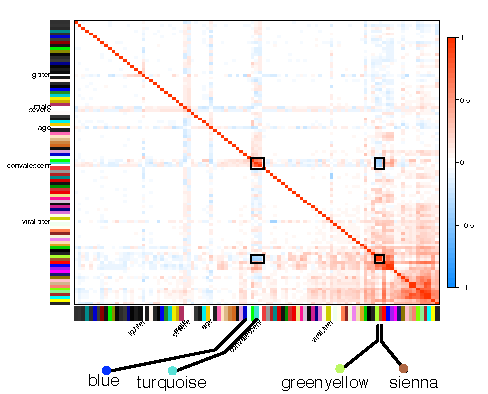
\includegraphics[width=\textwidth]{chap6/fig_7c_coEM_corr}
  \caption[Correlations between coexpression modules and clinical variables]{
  \textbf{Correlations between coEM eigengenes (colored bars on each axis) and the clinical variables (text labels).} The four coEMs from Figure \ref{fig:chik_TOM} are again highlighted here. There is a strong four-way relationship between the turquoise + convalescent vs.\ greenyellow + sienna nodes (black boxes). 
  }
  \label{fig:coEM_corr}
\end{figure}

We again utilized gene set enrichment analysis to explore the composition of these modules. The sienna module was most significantly enriched for GO, Reactome, and WikiPathways terms regarding the regulation of cytokine production, immune system signaling, and type II interferon signaling (Table \ref{tab:chik_coEM_enrichr}). The blue module was significantly enriched for broader terms regarding gene expression, infectious disease, and proteasome degradation. On the other hand, the greenyellow module did not achieve any significant enrichments among these annotation libraries at FDR < 0.1, and the size of the turquoise module (10,589 genes) precluded meaningful enrichment analysis.

\begin{figure*}[htb]
  \centering
  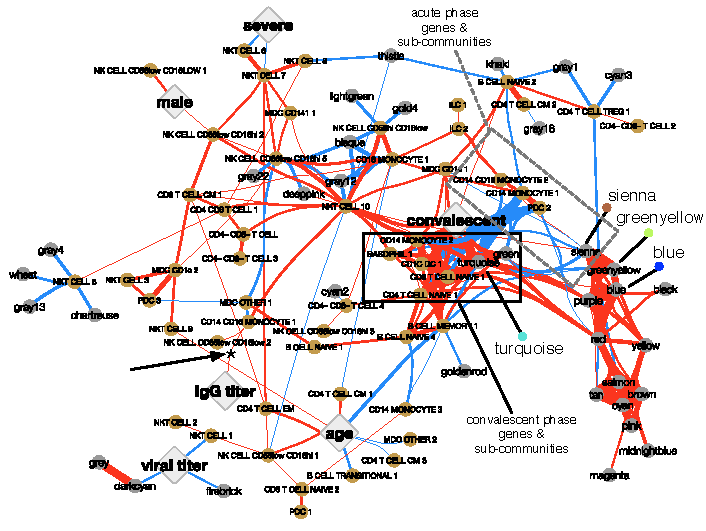
\includegraphics[width=\textwidth]{chap6/fig_7d_multiscale_network}
  \caption[Multiscale network of cell sub-community and coEM eigengenes]{
  \textbf{Multiscale network of cell sub-community and coEM eigengenes depicted with a force-directed layout and edge bundling.} Gold nodes, cell sub-communities; gray nodes, coEM eigengenes; large diamonds, clinical variables; red edges, positive correlations; blue edges, negative correlations. Edges are filtered to correlations significant at \emph{P} < 0.001, and thickness corresponds to the square of the correlations. A cluster of sub-communities and coEMs associated with convalescence (solid black box) and a corresponding cluster of sub-communities and coEMs associated with acute infection (dashed gray box) surround the “convalescent” node. A positive correlation between 15d post symptom onset CHIKV IgG titer and CD14+ CD16+ monocyte sub-community 1 (shown previously for acute phase samples in Figure \ref{fig:corr_cytof_igg}) is also visible (asterisk and arrow).
  }
  \label{fig:multiscale_network}
\end{figure*}

\newthought{To create} a multiscale model spanning all experimental measurements, we expanded the interaction network to include correlations with cell \subcommunity{} frequencies (from CyTOF) and serum cytokine concentrations (from Luminex). When adding the latter dataset, the large positive correlations between nearly all cytokine concentrations mentioned previously (Appendix Figures \ref{fig:corrplot_luminex_cytof_bothtimes}–\ref{fig:corrplot_luminex_cytof_conv}) created a large connected component dominating the network structure (Appendix Figure \ref{fig:multiscale_w_luminex}). Focusing on the transcriptomic and cell \subcommunity{} data and restricting to correlations significant at \emph{P} < 0.001, a well-organized network formed around the primary contrast in our dataset, the acute vs.\ convalescent timepoints (Figure \ref{fig:multiscale_network}). Under a force-directed layout, cell \subcommunities{} and gene modules that positively correlate with the convalescent timepoint clustered together (solid black box, Figure \ref{fig:multiscale_network}), while cell \subcommunities{} and gene modules that negatively correlate with convalescence (and therefore associate with acute infection) also clustered together (dashed gray box, Figure \ref{fig:multiscale_network}). Weaker correlations between other gene modules, cell \subcommunities{}, and the other clinical variables remained on the periphery of the network. For instance, the previously described significantly positive correlation between acute phase “nonclassical” CD14\sups{+}\allowbreak CD16\sups{++} monocytes (\subcommunity{} 1) and CHIKV IgG titer reappears as a weaker positive correlation (asterisk with arrow, Figure \ref{fig:multiscale_network}), since the network analysis includes both timepoints.

\begin{figure*}[htb]
  \centering
  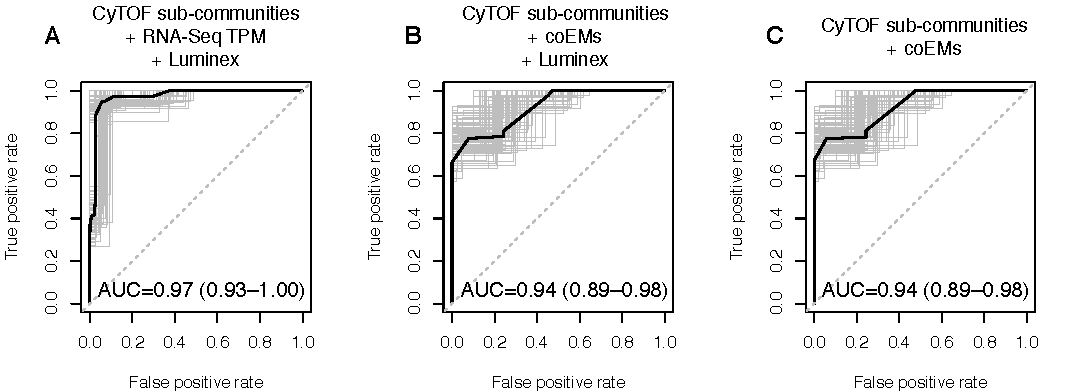
\includegraphics[width=\textwidth]{chap6/fig_S27_elasticnet}
  \caption[Performance of elastic net regression models for predicting timepoint]{
  \textbf{Receiver operator characteristic (ROC) curves measuring the performance of elastic net logistic regression models predicting the phase of infection} (acute vs. convalescent) for each sample, using progressively reduced versions of the dataset. Thin grey lines show the ROC curves for 100 bootstrap replicates. The area under the curve (AUC) along with its 95\% confidence interval are shown underneath each plot; a perfect classifier would achieve AUC=1 while a random classifier is expected to achieve AUC=0.5 (dashed diagonal line). A, model trained using all CyTOF sub-community frequencies, all quantified RNA-seq transcripts, and all Luminex cytokine measurements achieves near-perfect performance. B, model trained as in A with eigengene values for 92 coexpression modules replacing the RNA-seq transcript-level quantification; performance is slightly decreased but remains within the confidence interval for A’s AUC. C, model trained as in B with Luminex cytokine measurements removed; performance is equivalent to the model trained in B.
  }
  \label{fig:chik_elasticnet}
\end{figure*}

To test whether the severe dimensionality reduction of the three datasets to the relatively small network model presented in Figure \ref{fig:multiscale_network} retained predictive value for the acute-convalescent contrast, we fit elastic net regularized logistic regression models to three versions of the merged data: A, complete \pertranscript{} quantification, \subcommunity{} frequencies, and serum cytokine concentrations; B, same as A but with coEM eigengenes instead of \pertranscript{} quantification; and C, same as B but with serum cytokine concentrations removed, as in the final network model. As expected, given the strong transcriptomic signature for timepoint, the model that had access to complete \pertranscript{} quantification achieved nearly perfect performance under five-fold cross validation (area under the receiver operating characteristic [AUC]=0.97, 95\% confidence interval [CI] 0.93–1.00; Figure \ref{fig:chik_elasticnet}A). Replacing \pertranscript{} quantification with the 92 coEM eigengenes decreased predictive performance only slightly (AUC=0.94, 95\% CI 0.89–0.98; Figure \ref{fig:chik_elasticnet}B). Removing the serum cytokine data, leaving only the dimensionality-reduced data used to generate Fig 7D, did not further detract from model performance (AUC=0.94, 95\% CI 0.89–0.98; Figure \ref{fig:chik_elasticnet}C). This suggests that the compact, multiscale network model presented in Figure \ref{fig:multiscale_network} preserves the majority of the contrast between the two phases of infection profiled by our study.

\section{Discussion}

We present in this study the most comprehensive immune profiles available for natural human infections by CHIKV. By employing a diverse CyTOF antibody panel and novel clustering techniques to systematically discover \subcommunities{} and their frequencies in these data, we discovered more heterogeneity within PBMC populations than previously recognized in previous studies of viral infection. Considering the scarcity of any CyTOF data from viral infections,\autocite{Miner2015,Sen2015} these data may represent the most comprehensive immune profiles for any human viral disease. By taking an unbiased approach in measuring global changes across three scales (cell subpopulations, gene expression, and serum cytokines), we provide unprecedented robustness and detail on the effects of CHIKV on humans and a number of novel findings that compel future hypothesis-driven studies.

\subsection{Strong association of CHIKV and monocyte \subcommunities{}}

On the cell population level, our findings indicate a prominent role for CD14\sups{+} and CD14\sups{+}\allowbreak CD16\sups{+} monocytes—including several novel phenotypes therein—during the acute immune response to CHIKV. Two cell \subcommunities{} were more strongly associated with acute infection than all other \subcommunities{} by two orders of magnitude: “intermediate” CD14\sups{++}\allowbreak CD16\sups{+} monocytes and a CD123\sups{+}, CX3CR1\sups{+} and CD141\sups{+} subpopulation of CD14\sups{+} monocytes.	

“Intermediate” CD14\sups{++}\allowbreak CD16\sups{+} monocytes are a recently described population\autocite{Wong2011,Ziegler-Heitbrock2010} that received initial attention for showing independent predictive value for cardiovascular event risk,\autocite{Rogacev2012} which hinted at a role in vascular inflammation or atherosclerosis. They were also found to selectively express CCR5, the coreceptor for HIV.\autocite{Ellery2007} Subsequently, studies discovered that these cells are selectively (i.e., in contrast to “nonclassical” CD14\sups{+}\allowbreak CD16\sups{++} monocytes) expanded in bacterial sepsis, Dengue fever, Crohn’s disease, rheumatoid arthritis, Eale’s disease, and asthma.\autocite{Wong2012} Compared to our putative cluster of “nonclassical” CD14\sups{+}\allowbreak CD16\sups{++} monocytes, we too saw higher expression of CCR5 in the “intermediate” subpopulation, as well as higher expression of HLA-DR, another selective marker (Appendix Figure \ref{fig:cd14cd16_channel_diffs}), providing strong evidence that this population is the same “intermediate” phenotype described in previous studies.\autocite{Zawada2011} Very recently, in vitro studies were able to induce the “intermediate” phenotype from CD14\sups{+}\allowbreak CD16\sups{–} monocytes by treatment with IL-10,\autocite{Tsukamoto2017} a cytokine that we also found was elevated during acute infection (Figure \ref{fig:luminex}E). Since “intermediate” monocytes are known to be potent secretors of IL-10,\autocite{Skrzeczynska-Moncznik2008} a positive feedback loop involving IL-10 could contribute to the strong, selective expansion in “intermediate” monocytes that was observed during the acute phase. Given how much remains to be characterized about “intermediate” monocytes, and since they associate with inflammatory and autoimmune joint diseases that resemble chronic CHIKV arthropathy (like rheumatoid arthritis), this is an exciting avenue for further inquiry.\autocite{Chaaitanya2011,Miner2015,Fingerle1993,Nakaya2012}

Additionally, we discovered a novel subpopulation of CD14\sups{+} monocytes associating with the acute phase of infection that expressed high levels of CCR4, CXCR3 and CCR6, among other markers (Figure \ref{fig:subcomm_marker_diffs} and Appendix Figure \ref{fig:cd14_channel_diffs}). These markers have never been described in association with a distinct subpopulation of monocytes. This demonstrates that the heterogeneity of monocytes may extend beyond the “nonclassical”, “intermediate”, and “classical” divisions,\autocite{Appleby2013,Ziegler-Heitbrock2013} and that more careful identification of specific subpopulations will be needed to fully understand monocyte functionality.\autocite{Stansfield2015}

A globally significant correlation was found between “nonclassical” CD14\sups{+}\allowbreak CD16\sups{++} monocyte frequency at the acute phase and the CHIKV IgG titer two weeks later (Figure \ref{fig:corr_cytof_igg}). This suggests that this subpopulation could contribute to the development of a stronger humoral response, with potentially long-term implications, given an association discovered between the early IgG response and decreased likelihood of chronic arthralgia.\autocite{Kam2012} Recent studies have suggested that monocytes can have a role in modulating activation of certain T cells,\autocite{Charron2015,Eberl2009} which implies that monocyte subpopulations may contribute to the success of the adaptive immune response for certain pathogens. One study of this crosstalk reported induction of cytokines in δγ T cell–monocyte co-culture that closely matched the pattern of upregulation seen in our study, including IFNγ, TNFα, CCL2, IL-8, and CXCL10.\autocite{Eberl2009} Even more relevant is a recent study of in vitro infection of CD14\sups{+} monocytes by DENV, which upregulated CD16 expression and induced differentiation of B cells into plasmablasts, ultimately increasing IgG secretion.\autocite{Kwissa2014} Considering that this sequence of events closely mirrors the findings of our study, such as the high expression of CHIKV surface protein in monocytes, upregulation of CD14\sups{+}\allowbreak CD16\sups{+} monocytes during acute infection, and the correlation with convalescent phase IgG titers, a similar mechanism may apply equally to CHIKV pathogenesis.

\subsection{Serum cytokines support a monocyte-centric response to CHIKV}

In our study, most of the cytokines that were increased during acute infection were likely secreted by monocytes or contributed to the observed expansions of monocyte subpopulations (Figure \ref{fig:luminex}). The pronounced acute-phase increase in CXCL10, the most upregulated cytokine observed in our study, is likely linked to secretion by monocyte populations that expanded during the acute phase, since monocytes and T cells secrete CXCL10 in response to IFNγ.\autocite{Luster1987} CXCL10, which induces chemotaxis in monocytes, monocyte-derived cells, and T cells, can also be induced by IFNα and TNFα, which were upregulated in our study during the acute phase of infection.\autocite{Liu2011} Changes in CXCL10 expression are well-correlated with many infectious diseases,\autocite{Liu2011} although the role of CXCL10 in viral pathogenesis and its signalling pathways is still poorly understood (as it seems to alternately promote or protect against infection in different studies).	

In the previous section, we speculated that a feed-forward loop between production of IL-10 by “intermediate” CD14\sups{++}\allowbreak CD16\sups{+} monocytes\autocite{Skrzeczynska-Moncznik2008} and induction of the “intermediate” phenotype by IL-10\autocite{Tsukamoto2017} could help explain the upregulation of IL-10 during acute CHIKV infection. Another contribution could be from T cells, since monocyte–T cell interactions are able to activate T cells to an IL-10 secreting state.\autocite{Charron2015} IL-10 secretion is known to be dependent on a number of regulatory factors that were transcriptionally upregulated in our study, such as \emph{p38}, \emph{NF-κΒ}, and \emph{MyD88} (Appendix Figure \ref{fig:pathview_hsa04620}).\autocite{Saraiva2010} Another cytokine that likely contributed to the observed expansions in CD14\sups{+} and CD14\sups{+}\allowbreak CD16\sups{+} monocyte subpopulations is CCL2, a known CD14\sups{+} monocyte chemoattractant,\autocite{Serbina2008} which we observed to be upregulated during acute infection. CCL2 is secreted by monocytes and fibroblasts among many other cell types,\autocite{VanDamme1994} and like IL-10, its secretion from monocytes is also \emph{p38} and \emph{NF-κB} dependent.\autocite{Fietta2002} CCL2 was the only cytokine that positively correlated with all monocyte subpopulation frequencies during the convalescent timepoint, which significantly differed from the correlations observed for all other cytokines (Figure \ref{fig:luminex_monocyte_corr}). Finally, although we did not see significant upregulation of serum CCL7 levels, and the antibody panel did not include CCL8, RNA-seq did find that both of these genes were in fact transcriptionally upregulated during the acute phase (Figure \ref{fig:pathview_hsa04060}). These gene products are both CCR2-binding monocyte chemoattractants (although less well characterized than CCL2) and therefore may have also contributed to expansions in monocyte populations.

\newthought{Most previous studies} that profiled immunological changes associated with CHIKV in humans focused on serum cytokine levels.\sidecite[-1.5cm]{Chaaitanya2011,Chow2011,Ng2009,Schilte2013,Teng2015} Our results were largely concordant with previous studies, but there were also some notable differences. Of the significantly elevated cytokines in our data, CXCL10, CCL2, IFNα, IL-10, and IL-1Ra concur with the changes supported by a recent systematic meta-analysis of these studies.\autocite{Teng2015} We observed two changes that were not consistent, however. An increase in IL-8 was observed during the acute phase, although previous studies vary on whether it is upregulated or downregulated in the acute phase, and it may be in fact due to a dependency of the effect on viral load.\autocite{Teng2015} We also saw an increase in TNF-α, but very few previous studies included this cytokine.

The meta-analysis reports more cytokines that were upregulated during acute CHIKV infection than we observed, which might be expected given the increased power of combining several similarly sized previous studies. We often saw slight increases for these additional reported cytokines in our own data (e.g., IFNγ, IL-6, IL-15) but they did not reach statistical signficance in this study. One of the changes most consistently reported in the literature that was not replicated in our study was an upregulation of IL-6—we observed an upward shift that did not achieve statistical significance.\autocite{Chow2011,Ng2009} We also did not see globally significant associations between any cytokine levels and severity of symptoms, unlike previous studies.\autocite{Chow2011,Ng2009} This could be for any of a number of reasons: our statistical methods could be overly conservative, our cohort may have been too homogenous in symptomatology (the contrast between non-severe and severe cases was not emphasized during enrollment), or our cohort could simply differ too much from prior studies (adults vs.\ pediatric cases, differences in the CHIKV strain, or environmental differences). Reviews have already noted considerable variability in the results for serum cytokine studies on CHIKV,\autocite{Burt2017} suggesting that either much larger cohorts or a wider variety of immune profiling data will be needed to generate more reliable profiles. In part, this was a motivating factor for us to incorporate cell subpopulation and transcriptomic data into our immune profiles of CHIKV infection.

\subsection{Transcriptomic signatures for CHIKV infection phase, viremia, severity, and immunogenicity}

Our results are generally consistent with the transcriptomic signature recently reported for a C57BL/6J mouse model of CHIKV infection.\autocite{Wilson2017} We both find that the strongest acute phase transcriptional upregulation occurs in interferon-associated genes like IFI’s, \emph{MX1} and \emph{MX2}, \emph{OAS} genes, and \emph{RSAD2} (Viperin).\autocite{Wilson2017} Notably, in mice, \emph{CXCL10} and \emph{CXCL9} were the most upregulated cytokine genes when comparing the acute phase to controls, with \emph{CCL2} also substantially upregulated,\autocite{Wilson2017} mirroring our measurements of the most significantly modulated serum cytokine concentrations. Although not emphasized in their study, this reveals some consistency to the monocyte-\allowbreak centric immune response to CHIKV between mice and humans. Our finding that type I IFN genes are not upregulated during acute infection—while initially surprising since serum concentrations of IFNα were in fact elevated—turns out to be consistent with the mouse model, which found very low RNA abundance for type I IFN transcripts.\autocite{Wilson2017} Likewise, among IFN-regulated transcription factors, we find a concordant pattern of \emph{IRF7} and \emph{IRF9} upregulation during the acute phase, while \emph{IRF3} is not upregulated (Appendix Figure \ref{fig:pathview_hsa05164}). Together, these data establish that this mouse model of CHIKV replicates many aspects of the gene expression signature induced by CHIKV in humans, including modulations of interferon pathways and monocyte-related cytokines, and therefore support its continued use as a model of human CHIKV pathogenesis and the corresponding innate immune response.

Besides a large acute-convalescent transcriptomic signature, we were also able to elucidate three novel transcriptomic signatures for CHIKV viral titer, symptom severity and the convalescent phase CHIKV IgG titer. This was aided by the use of transcript-level quantification and statistical models that incorporate the uncertainty of the quantification process.\autocite{Pimentel2016} Notably, these signatures were constructed after incorporating timepoint as a covariate—i.e., they were found to significantly add information to a model that had already accounted for timepoint, age, and gender. Of these signatures, the strongest and least surprising was the signature for higher acute phase CHIKV viral titer, which was enriched for cytokine signalling, leukocyte activation, and interferon signaling genes. The presence of a distinct signature for viral titer in our data indicates that a more viremic acute phase must have led to transcriptional upregulation of these genes across both timepoints, otherwise they would be sufficiently captured by the acute-convalescent DET signature alone.

The transcriptional signatures for symptom severity and immunogenicity were notable for having an abundance of HLA (aka major histocompatibility complex [MHC]) transcripts—in particular, \emph{HLA-A}, \emph{HLA-B}, and \emph{HLA-DOB}. Our study showed that certain \emph{HLA-B} transcripts appeared to be associated with less severe acute phase symptoms (Figures \ref{fig:DET_severity_volcano}–\ref{fig:DET_severity_boxplot}), while certain \emph{HLA-A} and \emph{HLA-DOB} transcripts were correlated with changes in the 15d CHIKV IgG titer (Figure \ref{fig:DET_IgG_volcano}). It is not surprising that HLA gene expression could affect infection outcomes, since the HLAs are responsible for antigen presentation and both the adaptive and cellular immune responses. For instance, during viral infection, IFNα and IFNγ increases the transcription of MHC class I loci and \emph{HLA-B} in particular,\autocite{Girdlestone1995} so we could speculate from our data that a particularly strong \emph{HLA-B} response boosts the cytotoxic immune response and mitigates acute phase symptoms. Based on known roles for MHCs it is also reasonable that more transcription of \emph{HLA-A} (a class I allele) would correlate with lower IgG titers, while more transcription of \emph{HLA-DOB} (a class II allele) would correlate with higher IgG titers (Figure \ref{fig:DET_IgG_volcano}), since the former initiates the cytotoxic (non-humoral) response while the latter is involved in the adaptive and humoral responses. Our data, therefore, could be interpreted to reflect different relative prioritization of these immune responses among our cohorts’ patients that manifests as a difference in magnitude of the early IgG response, which was previously observed to correlate with decreased risk of chronic arthralgia.\autocite{Kam2012} Since allelic diversity in HLA loci are well-established genetic risk factors for certain infectious and autoimmune diseases, our signatures may also reflect underlying genetic variation (e.g., expression quantitative trait loci) that affects transcription of HLA genes and thereby shifts disease outcomes.\autocite{Kumar2014} Finding host genetic factors for CHIKV severity could lead to further insight into mechanisms of pathogenesis, so this is a promising direction for future study.

\subsection{A multiscale network model of CHIKV pathogenesis}

Finally, our study generated a network model that integrates global measurements of cell \subcommunities{}, cytokines, and gene transcription into a compact roadmap of the immune responses triggered by CHIKV (Figure \ref{fig:multiscale_network}). A network that leverages modularity is valuable because of the inherent limitations of gene-level or cell-level analyses, which are poorly suited for traditional inference testing or Bayesian analysis because of their high dimensionality and non-independence among many of the observations. To our knowledge, we are the first to attempt a combination of WGCNA for detecting transcriptional network modularity with comprehensive cell \subcommunity{} frequencies modeled within CyTOF data. 

WGCNA produced 92 coexpression gene modules, four of which were significantly enriched for DET signatures for either infection phase or viral titer. One of these coEMs, sienna (426 genes), was significantly enriched for cytokine signalling and immune signalling terms and correlated with the acute phase of infection; a second much larger module, turquoise (10,589 genes), strongly correlated with the convalescent phase of infection. Combining gene modules with subpopulation frequencies and serum cytokine concentrations into a correlational network and filtering for edges at \emph{P} < 0.001 produced a network dominated by intracorrelation in the cytokines (Appendix Figure \ref{fig:multiscale_w_luminex}). Since none of the cytokines correlate significantly with the clinical variables, we removed them from the network to produce a more compact model (Figure \ref{fig:multiscale_network}). Under a force-directed layout, this network organizes around the primary contrast in our data—the phase of infection—with acute phase vs.\ convalescent phase genes and cell subpopulations separating into two communities. The sienna module also serves as a “bridge” between the timepoint contrast and most of the other strong interactions between gene modules in our dataset.

Although limited by sample size and the specific timepoints used in our study, this network represents the first completely data-driven model of the immune reaction to CHIKV across multiple layers of “omic” data. It compactly summarizes changes of hundreds of thousands of measured analytes with minimal reduction in the predictive value for the timepoint contrast (Fig \ref{fig:chik_elasticnet}), and puts these interactions into global context with other clinical variables. We hope that the generation of similar multiscale networks for other viral infections, e.g., Dengue and Zika, will soon lend insight into the comparative effects of these viruses on the human immune system and aid in the discovery of therapeutics and prognostic biomarkers that remain robust across the multiplicity of arboviral infections now prevalent in tropical urban regions.

\subsection{Conclusions}

Our comprehensive immune profiling of 42 pediatric cases of CHIKV infection revealed an immune response largely centered on changes in monocyte subpopulations and monocyte-related cytokines. Monocytes displayed the highest change in CHIKV surface protein expression between the two timepoints. An “intermediate” CD14\sups{++}\allowbreak CD16\sups{+} subpopulation and an activated (CD123\sups{+}, CX3CR1\sups{+} and CD141\sups{+}) CD14\sups{+} monocyte subpopulation associated most strong\-ly with the acute phase of infection when compared against all other identified subpopulations of PBMCs. Interestingly, we also found a subpopulation of CD14\sups{+} monocytes with distinctly higher expression of previously unreported markers (CCR4, CXCR3 and CCR6) that also associated with the acute phase of infection. Although “nonclassical” CD14\sups{+}\allowbreak CD16\sups{++} monocyte frequencies were unchanged across the timepoints, we found a significant correlation between their frequency at the acute phase and corresponding convalescent phase CHIKV IgG titers. Finally, among the elevated serum cytokine levels for the acute phase of infection, half concerned known monocyte chemoattractants (CXCL10, CCL2, and IL-10).

Our study produced additional novel findings. We confirmed that transcriptomic effects of CHIKV in humans for the different phases of infection correspond well to those recently reported for a mouse model,\autocite{Wilson2017} but furthermore, we discovered new transcriptomic signatures for the level of acute phase viremia, acute phase symptom severity, and convalescent phase immunogenicity. Among the signatures for acute severity and convalescent immunogenicity, we found an abundance of specific HLA transcripts that correlated with both of these outcomes, and a notably strong correlation between severity and transcription of \emph{MXRA7}, an essentially uncharacterized gene with only two unrelated disease associations reported in the literature.\autocite{Sim2013,Veiga-Castelli2010} We also find globally significant expression of CHIKV surface protein on several B cell subpopulations, which have never been productively infected in vitro by CHIKV.\autocite{Her2010,Sourisseau2007,Teng2012a} Finally, we have integrated all of our observed changes into a multiscale network that summarizes the immunological changes across the cellular and gene expression levels and their interactions with certain clinical outcomes. We hope that our findings have provided a uniquely global perspective on the biomolecular landscape of CHIK pathophysiology, and that they spark new hypotheses for future experiments that can further disentangle the mechanisms of CHIKV pathogenesis and the components of a successful immune response in humans.

\section{Materials and Methods}

\subsection{Study participants}

To characterize immune profiles of CHIKV infection, 43 chikungunya cases (42 for analysis plus one extra) were selected from the participants aged 6 months to 14 years who were enrolled in our ongoing study at the National Pediatric Reference Hospital (HIMJR) in Managua, Nicaragua between September 2015 and April 2016. Chikungunya cases were laboratory-confirmed by detection of CHIKV using RT-PCR/virus isolation in acute-phase samples, seroconversion by IgM capture ELISA and/or a >4-fold increase in antibody titer by Inhibition ELISA in paired acute and convalescent sera.\autocite{Balmaseda2006,Hammond2005} Participants were also screened for dengue virus (DENV) infection, and CHIKV/DENV co-infections were excluded. To obtain a homogenous set of samples, all selected cases had an acute-phase sample collected on days 2-3 of illness and a convalescent sample collected on days 15-17 post-illness for plasma, whole blood in PAXgene solution, and peripheral blood mononuclear cells (PBMCs). PBMCs were isolated from whole blood as previously described.\autocite{Zompi2012} Clinical information was collected every 12 hours, and was digitized by double-data entry under systematic monitoring by a clinical supervisor, with quality control checks performed daily and weekly. 

\subsection{CyTOF sample processing and acquisition}

Cryopreserved PBMC samples from the acute and convalescent phases of infection were thawed and stained with Rh103 nucleic acid intercalator (Fluidigm) as a viability marker. Paired PBMC samples from each timepoint were first barcoded using a CD45 antibody-based barcoding approach,\autocite{Mei2016} and each acute and convalescent sample pair was pooled as a single patient sample for subsequent processing to minimize technical variability and potential batch effects. The pooled patient samples were then stained with a validated 37-marker CyTOF antibody panel (Appendix Table \ref{tab:chik_antibodies}) for 30 minutes on ice and then fixed, permeabilized and incubated with Ir nucleic acid intercalator (Fluidigm). The samples were then stored in freshly-diluted 2\% formaldehyde in PBS and stored until acquisition. Immediately prior to CyTOF acquisition, the samples were washed with deionized water (diH20), counted and resuspended in diH20 containing a 1/20 dilution of Eq 4 Element beads (Fluidigm). Following routine autotuning, the samples were acquired on a CyTOF2 mass cytometer (Fluidigm) equipped with a SuperSampler fluidics system (Victorian Airships) at an event rate of <400 Hz. 

\subsection{CyTOF data analysis}

Following data acquisition, the FCS files were normalized using the bead-based normalization algorithm in the CyTOF control software, and uploaded to Cytobank for initial data processing. Normalization beads were excluded based on Ce140 signal, and cell events were identified based on Ir191/193 DNA signal. A conservative doublet exclusion gate was applied based on DNA and event length, and Rh103\sups{+} dead cells were also excluded. The cell events associated with the acute and convalescent samples were then manually de-barcoded based on CD45-194Pt and CD45-198Pt expression, respectively, and were split and exported as separate samples for subsequent analyses using a semi-supervised computational analysis pipeline. 

We first applied traditional hierarchical gating to a subset of samples to identify 9 major immune compartments: CD4\sups{+} and CD8\sups{+} T cells, B cells, NK cells, NKT cells, Monocytes, mDCs, pDCs, and basophils. This manually gated data was used to train a logistic regression classifier (which we term \texttt{Nod}), which was then applied to identify these populations in all the samples. We then applied Phenograph\autocite{Levine2015a} as an unbiased approach to define the phenotypic heterogeneity within each of these compartments (\texttt{HybridLouvain}). The cell clusters identified in each single sample were then meta-clustered across all samples to identify phenotypically-similar communities that were reproducibly present across multiple samples (\texttt{MetaHybridLouvain}). These meta-clusters were then manually annotated based on overall marker expression profiles and their association with known immune cell subsets, allowing for the presence of additional phenotypically distinct sub-clusters within these known subsets. These annotations were mapped back to the individual samples, and the relative frequency and median marker expression patterns of these consistently annotated clusters were then exported for further statistical analyses. Metaclusters that were characterized by protein expression patterns that did not correspond to any known cell subsets, including those that appeared to be cell-cell doublets, were annotated as “undefined” and not included in subsequent statistical or network analyses.

\subsection{Multiplex ELISA}

Cytokines and chemokines were measured using a multiplex ELISA-based assay (Luminex). All serum samples were inactivated with a UV-C lamp (254 nm) for 10 min on ice in a biosafety-level 3 laboratory at the University of California, Berkeley. Each sample was run in duplicate in a 96-well micro titer plate using 25 μL of plasma or serum from each patient from acute and convalescent time points using the multiplex cytokine panels (Multiplex High Sensitivity Human Cytokine Panel, Millipore Corp.). 41 analytes (cytokines and chemokines) were measured measured using a Luminex-200 system and the XMap Platform (Luminex Corporation). Acquired mean fluorescence data was analyzed and calculated by the Beadview software. The lower and upper detection limits for these assays are 3.0 pg/mL and 15,000 pg/mL, respectively. Quality control of each sample was performed and samples with bead counts <50 were not used for analysis.  

\subsection{Viral titer assays}

Viral RNA was extracted from 140 μL of cell culture supernatant or 140 μL of patient serum using the QIAamp Viral RNA Mini Kit (Qiagen) according to the manufacturer’s protocol, and RNA was eluted in 60 μL of RNase-free water. Primers for the E1 gene were designed to quantify CHIKV copies in each patient and were used at 300 nM final concentration. The forward primer is 5'-\texttt{\seqsplit{CATCTGCACYCAAGTGTACCA}}-3' and the reverse primer is 5'-\texttt{\seqsplit{GCGCATTTTGCCTTCGTAATG}}-3'.  A TaqMan labeled probe was used for detection: FAM-\texttt{\seqsplit{GCGGTGTACACTGCCTGTGACYGC}}-BHQ-1. The SuperScript III One-Step RT-PCR System (Invitrogen) was used for reverse transcription of viral RNA and subsequent amplification of viral complementary DNA (cDNA). Specifically, 5 μL of extracted viral RNA, 0.5 μL of SuperScript III RT/Platinum Taq High Fidelity Enzyme Mix (Invitrogen), 12.5 μL of 2× Reaction buffer, 5 μL RNase free water and 2 μL of primers and probes were added to each well. Viral RNA was reverse transcribed (52°C for 15 minutes), and the resulting cDNA was amplified via one cycle of denaturation (94°C for 2 minutes), 45 cycles of denaturation (94°C for 15 seconds), annealing (55°C for 40 seconds), and extension (68°C for 10 seconds). For quantitation of CHIKV copies, a 4-point standard curve (8.0, 6.0, 4.0, and 2.0 log\subs{10} copies/μL of eluate) was used. Standard curves were prepared using quantitated ssDNA (Integrated DNA Technologies) containing the target sequence of CHIKV with the following sequence: \texttt{\seqsplit{CACAACATCTGCACCCAAGTGTACCACAAAAGTATCTCCAGGCGGTGTACACTGCCTGTGACCGCCATTGTGTCATCGTTGCATTACGAAGGCAAAATGCGCACTAC}}

\subsection{Preparation of RNA sequencing libraries}

Total RNA was extracted from PaxGene RNA blood with the PAXgene Blood RNA Kit (Qiagen) by following manufacturers’ instructions including DNAse digestion and an additional clean-up using RNEasy MinElute kit (Qiagen). Purified RNA samples were quantified by Qubit 3.0 fluorometer with RNA High Sensitivity Assay kit (Thermo-Fisher). The quality of the RNA was confirmed by TapeStation 2200 with the RNA High Sensitivity ScreenTape (Agilent Technologies). To prepare the 84 samples’ libraries, ribosomal RNA (rRNA) and globin mRNA were removed from 200ng total RNA, and the remaining RNA was fragmented and primed for cDNA synthesis using TruSeq Total Stranded RNA HT kit with Ribo-Zero Globin on a Microlab STAR automated liquid handling system (Hamilton). The libraries were barcoded with TruSeq HT indices to allow for multiplexing and ligation-mediated PCR was performed to enrich barcoded libraries for 15 cycles, then purified with the Agencourt AMPure XP beads system (Beckman Coulter). The libraries were assessed for quality with the high sensitivity DNA chip in a TapeStation 2200 (Agilent) and quantified with KAPA Library Quantification Kits for Illumina platforms (Kapa Biosystems). The libraries were diluted to 2nM and combined equimolarly in pools of 12. These pools were then clustered using a cBot (Illumina) with a HiSeq 3000/4000 paired-end cluster kit on a patterned flow cell, one pool per lane. The flow cell was sequenced on a HiSeq4000 using a HiSeq 3000/4000 SBS kit (300 cycles, Illumina). Two technical replicates were sequenced per biological sample for a total of 168 sequencing runs.

\subsection{Pre-processing of RNA-seq data}

Sequencer-generated base call (BCL) files were converted to FASTQ files and the multiplexed samples were separated using \texttt{bcl2fastq}, which was then assessed for sequencing quality using FastQC\footnote{\url{http://www.bioinformatics.babraham.ac.uk/projects/fastqc/}} (version 0.11.4) to assess the quality of the sequencing data. The FASTQ files were quality filtered by using FASTAX Toolkit\footnote{\url{http://hannonlab.cshl.edu/fastx\textunderscore toolkit/}} with the invocation \texttt{fastq\textunderscore quality\textunderscore filter -q 30 -p 50 -v -Q 33}, and only the sequencing reads that met all quality control requirements were aligned to the latest human reference genome (GRCh38) using HISAT2\autocite{Kim2015} (version 2.0.4). SAMtools\autocite{Li2009b} (version 0.1.19) was used to sort and convert the SAM files to BAM. Aligned sequences were assembled into potential transcripts using StringTie\autocite{Pertea2015} (version 1.2.2). SAM files of preprocessed RNA-seq alignments were also analyzed with the \texttt{htseq-count} script from HTseq\autocite{Anders2015} for differential expression analysis by counting the overlap of reads with genes.

\subsection{Differential expression analyses}

The assembled transcripts, representing the different splice variants for each gene locus, were quantified in order to analyze differential expression in response to CHIKV infection. Differentially expressed genes were analyzed using the R packages \texttt{ballgown}\autocite{Frazee2014,Pertea2016} and \texttt{DESeq2},\autocite{Anders2010} and the results were consolidated to increased robustness. The samples were compared between acute and convalescent timepoints with gender, age, and infection severity included as covariates. Pathway-based visualization of differentially expressed genes was performed with the \texttt{pathview}\autocite{Luo2013} R package and KEGG\autocite{Ogata1999} annotations.

For differential expression analysis at the transcript level, we used \texttt{kallisto}\autocite{Bray2016} (version 0.43.0) and \texttt{sleuth}\autocite{Pimentel2016} (version 0.28.1). These methods, based on pseudoalignment counts, are more computationally efficient than complete alignment methods and can use bootstrap replicates to model uncertainty at the quantification step.\autocite{Bray2016} Uncertainty in quantification is caused by the inherent ambiguity of assigning reads to transcripts and constrains other methods that use invariant transcript counts, whereas \texttt{sleuth}’s method can maintain sensitivity at the isoform level while adequately controlling the FDR.\autocite{Pimentel2016} Pseudoalignment utilized a transcriptome index built from Ensembl release 79 (March 2015) for GRCh38. \texttt{sleuth} uses an additive response error model under which each variable or covariate has fixed effects $\beta$ on each transcript’s abundance, and to determine significance, the Wald test was used for the null hypothesis that $\beta_t = 0$ for each transcript $t$. For the acute vs.\ convalescent (timepoint) signature, age and gender were included as covariates in the model, while for the viral titer, severity, and 15d IgG titer signatures, timepoint, age, and gender were included as covariates in the model. Viral titers and 15d IgG titers were modeled in units of log\subs{10} dilutions. All inference tests for differential expression analyses were adjusted for multiple hypotheses using the Benjamini-Hochberg procedure for controlling FDR.\autocite{Benjamini2001}

\subsection{Construction of gene coexpression networks and coexpression modules}

Gene coexpression networks were constructed from the gene-level expression data for all samples using weighted gene coexpression network analysis (WGCNA) using the \texttt{WGCNA}\autocite{Zhang2005} (version 1.51) and \texttt{coexpp}\footnote{\url{https://bitbucket.org/multiscale/coexpp}} (version 0.1.0) R packages. WGCNA leverages natural variance in expression between sampled individuals and timepoints to build a network structure from the Pearson correlations for all gene-gene pairs.\autocite{Zhang2005} \texttt{coexpp} is a specialized implementation of WGCNA that optimizes memory and multicore usage. Gene expression data were preprocessed for WGCNA by applying a log\subs{2} transformation to the FPKM quantification and removing the lowest-variance quartile of genes.\footnote[][-1.5cm]{WGCNA's use of Pearson's $r$ does not require assuming the data are normally distributed. \textcite{Nefzger1957} note that this is a needless assumption, and \textcite{Edgell1984} demonstrate that Pearson's $r$ is generally robust to non-normality for $N$ ≥ 15. Furthermore, \textcite{Allen2012} show that with non-normal (bimodal) data, WGCNA still outperforms Bayesian and partial correlation network reconstruction methods.} In our study, we did not normalize each timepoint separately, as we were interested in correlations across the timepoints and interactions between gene modules and the phase of infection.\footnote{A network describing correlations within each timepoint that remain unchanged across timepoints would result from standardizing acute and convalescent data separately. For more details on preparing RNA-seq and heterogeneous data for WGCNA, see Langfelder and Horvath's FAQ at \url{https://goo.gl/LU88Df}.} WGCNA then converts the gene-gene correlation matrix into an adjacency matrix using a power function that optimizes for scale-free topology, and adjacencies are then transformed into a topological overlap matrix (TOM) that represents normalized counts of neighbors that are shared between the nodes on either side of each edge. Genes were grouped using average-linkage hierarchical clustering of the TOM, followed by a dynamic cut-tree algorithm\autocite{Langfelder2008} that divides the dendrogram branches into gene coexpression network modules (coEMs). Relationships among coEMs and the other data were evaluated using eigengenes\autocite{Langfelder2007} (the first principal component of each coEM), calculating the Pearson correlations for all possible pairings of the coEM eigengenes, clinical variables, and cell subpopulations. Network layout was performed using the ForceAtlas2 algorithm in Gephi\autocite{Bastian2009} (version 0.9.1) followed by visualization in Cytoscape\autocite{Smoot2011} (version 3.4.0).

\subsection{Gene set enrichment analyses}

The acute-convalescent and viral titer DET signatures were analyzed for enrichment of Gene Ontology (GO) biological process\sidecite[-0.7cm]{GOC2015} (2015), Panther\autocite{Mi2013} (2016), and Reactome\autocite{Fabregat2016} (2016) terms using the Enrichr platform.\autocite{Chen2013} DETs were ranked by \emph{q} value, and query sets for Enrichr were created from the 100, 300, 1,000, and 3,000 top ranked DETs (all having \emph{q} < 0.05) mapped to unique gene symbols, which all produced qualitatively similar results for top enriched terms; representative results for 1,000 DETs are presented in this study. Enrichr improves on the typical method of ranking term significance with one-sided Fisher’s exact tests by multiplying their log-scaled \emph{P} values by a \emph{Z}-score of the deviation from the expected rank for each term, which decreases the bias of the Fisher’s exact method toward terms with few gene assignments.\autocite{Chen2013} Enrichment of WGCNA coEMs for terms from GO biological process (2015), Reactome (2016), and WikiPathways\autocite{Kutmon2016} (2016) was similarly calculated using Enrichr without ranking or cutoffs. Enrichment of DET signatures within each coEM was calculated using one-sided Fisher’s exact tests and a Benjamini-Hochberg adjustment.

\subsection{Data availability}

Raw RNA-seq reads and differentially expressed genes were deposited in GEO under study accession number \href{https://www.ncbi.nlm.nih.gov/geo/query/acc.cgi?acc=GSE99992}{GSE99992}.

\subsection{Statistical analyses}

Inference testing for unpaired quantitative variables\footnote{Although the study design is paired across timepoints, \texttt{MetaHybridLouvain}'s inability to identify every \subcommunity{} in all samples creates null values that complicate traditional paired analysis. Additionally, it is not possible to regress traditional linear models if patient ID is a covariate while also modeling the effects of per-patient covariates like gender, severity, and IgG titer (the design matrix will be rank deficient). One potential solution is to used mixed-effect models as implemented in limma-voom—see \textcite{Ritchie2015} and \textcite{Law2014}—which can model a random effect (as a varying intercept) for differences between patients. The downsides of this approach, both of which can result in decreased power, are the additional model degrees of freedom and limma-voom's inability to model the uncertainty of the quantification step provided by the \texttt{kallisto} bootstraps. Nevertheless, a repeat analysis using these models as implemented in the limma-voom framework by collaborators Mayte Suarez-Fariñas and Maria Suprun has recapitulated the major results of this chapter, and will be included in the submitted publication.} (CyTOF community and \subcommunity{} frequencies, marker expression means per \subcommunity{} per sample, and correlations between monocyte \subcommunity{} frequencies and Luminex analyte concentrations) used the Mann-Whitney \emph{U}, while the Wilcoxon signed-rank test was used for paired comparisons (Luminex analyte concentrations). Hypothesis testing for correlations used either Spearman's $\rho$ (\subcommunity{} frequencies vs.\ viral and IgG titers) or Pearson’s \emph{r} (multiscale network analysis). Visualization of small correlation matrices was performed with the \texttt{corrplot} R package. \emph{P} values in this study were adjusted for multiple hypotheses using either the Bonferroni or Benjamini-Hochberg (FDR-based aka \emph{q} value) methods, as specified throughout the Results. Elastic net regularized regression, which fits a logistic regression model with $\ell_1$ and $\ell_1$ penalties (the elastic net penalty), was performed with the \texttt{glmnet}\autocite{Friedman2010} R package (version 2.0-5). Elastic net hyper-parameters $\alpha$ and $\lambda$ were both selected empirically per model by a grid search that maximized AUC under five-fold nested cross validation. 100 bootstrap resampling runs were used to estimate the 95\% confidence interval for the AUC. R version 3.2.2 was used for all statistical analyses, and in addition to those already mentioned, the following package versions were used: \texttt{ggplot2} (2.2.1), \texttt{pheatmap} (1.0.8), \texttt{ROCR}\autocite{Sing2005} (1.0-7), and \texttt{Biobase} (2.30.0).

\section*{Notes}

\subsection*{Contributors}

Theodore R. Pak (\smallcaps{TRP}), Daniela Michlmayr (\smallcaps{DM}), Adeeb H. Rahman (\smallcaps{AHR}), El-Ad David Amir (\smallcaps{EDA}), Eun-Young Kim (\smallcaps{EK}), Angel Balmaseda (\smallcaps{AB}), Seunghee Kim-Schulze (\smallcaps{SKS}), Michael G. Stewart (\smallcaps{MGS}), Guajira P. Thomas (\smallcaps{GPT}), Steven Wolinsky (\smallcaps{SW}), Andrew Kasarskis (\smallcaps{AK}), and Eva Harris (\smallcaps{EH}) contributed to this chapter. 

\smallcaps{TRP}, \smallcaps{DM}, \smallcaps{AHR}, \smallcaps{SW}, \smallcaps{AK}, and \smallcaps{EH} designed the study. \smallcaps{EH} and \smallcaps{AB} directed studies in Nicaragua to obtain the samples for this study. \smallcaps{AHR} and \smallcaps{SKS} performed the CyTOF experiments. \smallcaps{AHR}, \smallcaps{SKS}, and \smallcaps{EDA} performed manual gating of CyTOF data, clustered events with \texttt{MetaHybridLouvain}, and created the viSNE plots within Figures \ref{fig:nodlabel_diag}, \ref{fig:mhl_visne}, and \ref{fig:chikv_visne}. \smallcaps{AHR} wrote the first draft of the CyTOF Methods subsections. \smallcaps{EH} and \smallcaps{DM} selected study participants; \smallcaps{DM} analyzed demographic data, performed the viral titer assays, and wrote the first draft of the corresponding Methods subsections and Table \ref{fig:chikv_visne}. \smallcaps{DM} and \smallcaps{SKS} performed Luminex assays. \smallcaps{EK}, \smallcaps{MGS}, and \smallcaps{GPT} prepared RNA-seq libraries, performed the sequencing, pre-processed the data, analyzed differentially expressed genes, and wrote the first draft of the corresponding Methods subsections. \smallcaps{TRP} analyzed differentially expressed transcripts, constructed network and predictive models, and performed statistical analyses. \smallcaps{TRP} created all other figures in this chapter and the Appendix and wrote the first draft of all other sections of this chapter. \smallcaps{TRP} and \smallcaps{DM} share first authorship on the manuscript for submission.

\subsection*{Funding}

This work was supported by NIH/NIAID grants U19-AI118610 (\smallcaps{TRP}, \smallcaps{DM}, \smallcaps{EH}, \smallcaps{AK}, \smallcaps{AHR}, \smallcaps{SW}), R33-AI100186 (\smallcaps{AB}, \smallcaps{EH}), F30-AI122673 (\smallcaps{TRP}), and in part by the resources and expertise of the Department of Scientific Computing at the Icahn School of Medicine at Mount Sinai. We thank study personnel at the HIMJR and the National Virology Laboratory of the Ministry of Health in Managua, Nicaragua for enrolling patients, collecting blood samples and clinical data, maintaining databases and a high level of quality control, and preparing PBMCs. We are grateful to the study participants and their families. The content is solely the responsibility of the authors and does not necessarily represent the official views of NIH.

\subsection*{Conflict of Interest}

The authors have no conflicts of interest to disclose.

\subsection*{Acknowledgements}

This work was supported in part by the resources and expertise of the Department of Scientific Computing at the Icahn School of Medicine at Mount Sinai. We thank Mayte Suarez-Fariñas and Maria Suprun for performing a confirmatory analysis using alternative statistical methods (such as mixed-effect models) and incorporating data from a repeat Luminex experiment, which reaffirmed the major findings in this chapter after the dissertation was defended. We thank study personnel at the HIMJR and the National Virology Laboratory of the Ministry of Health in Managua, Nicaragua for enrolling patients, collecting blood samples and clinical data, maintaining databases and a high level of quality control, and preparing PBMCs. We are grateful to the study participants and their families. We thank Ana Fernandez-Sesma and Irene Ramos-Lopez and all members of the Dengue Human Immune Profiling Consortium for their assistance in designing and conducting the study and their feedback on preliminary results.